% !Mode:: "TeX:UTF-8"
%!TEX program  = xelatex

%\documentclass[bwprint]{cumcmthesis}
\documentclass[withoutpreface,bwprint]{cumcmthesis} %去掉封面与编号页

\usepackage{float}	%用于排版图片位置
\usepackage{caption}	%用于 \captionof 命令
\usepackage{multirow}
\usepackage{array}
\usepackage{booktabs}
\usepackage{adjustbox}
\usepackage{url}
\usepackage{lmodern}

%需要核对承诺书和编号页
\title{多波束测深条带覆盖宽度建模与最优测线布设}
%\tihao{B}
%\baominghao{}
%\schoolname{西安电子科技大学}
%\membera{谷理想}
%\memberb{卫健康}
%\memberc{石智中}
%\supervisor{无}
%\yearinput{2026}
%\monthinput{05}
%\dayinput{05}

% 修复 cumcmthesis.cls 中 colorlinks + pdfborder 同时启用导致的 \ref 解析失败
\hypersetup{colorlinks=false, hidelinks}

% 抑制模板中 cleardoublepage 产生的空白页
\let\cleardoublepage\clearpage

\begin{document}

\maketitle
\begin{abstract}
本文针对多波束测深系统的条带覆盖宽度计算与测线布设优化问题，
基于波束与海底坡面的空间几何关系建立覆盖宽度解析模型，
并针对平面坡与真实测量地形两种场景分别设计了测线布设方案，
在保证全覆盖与重叠率约束的前提下最小化测线总长度，
实现了全覆盖、低重叠率与最短测线的多目标优化。

针对问题一，在测线与坡面走向垂直的截面内，由波束边缘射线与海底坡面求交，
建立覆盖宽度解析模型 $W = D\big[\frac{1}{\tan30^\circ+\tan\alpha}+\frac{1}{\tan30^\circ-\tan\alpha}\big]$，
并明确了重叠率按相邻条带中较窄者（瓶颈）计算的判定准则。
对 9 条测线（间距 200m）逐点计算：覆盖宽度自深水侧 315.71m 单调递减至浅水侧 170.27m，
重叠率由 32.78\% 递减至负值，浅水区出现 11.55m 与 29.73m 的覆盖空隙，
定量揭示了固定测线间距下浅水区成为覆盖瓶颈的机理。

针对问题二，将问题一模型推广至任意测线方向：引入视坡角 $\tan\alpha'=\tan\alpha|\sin\beta|$
刻画测线方向与坡面走向的空间关系，建立 $W(L,\beta)$ 的解析表达式，
计算 $L=0\sim2.1$ 海里、$\beta=0^\circ\sim315^\circ$ 的 $8\times8$ 覆盖宽度表（62.9$\sim$768.5m），
并指出 $\beta=90^\circ$（沿等深线方向）时覆盖宽度不随 $L$ 变化且最大，
为问题三的测线方向选择提供了直接依据。

针对问题三，设计“方向扫描—间距递推—全覆盖验证”的三步布设框架：
以 $\beta\in[0^\circ,180^\circ]$ 的相对总长扫描证明 $\beta=90^\circ$（沿等深线）总长最短，
东西向测线总长为其 5.69 倍；由重叠率约束 $10\%\le\eta\le20\%$ 反解得出间距上限
$d_i=0.9\,W_{\min}$，并解析递推全部测线位置，得 36 条南北向测线、总长 72 海里、
相邻条带重叠率恰为 10\%，动态规划验证其为约束下的最优方案。
进一步计入蛇形折返转弯段，完整航迹约 78 海里（保守估计 84.3 海里），
并给出重叠率下界敏感性分析（每放宽 5\% 约增 1 条测线）。

针对问题四，基于附件单波束测深数据（251$\times$201 网格，丘陵型地形，等深线方向标准差 50.6°），
建立方向相关的条带宽度场与测线方向扫描方法，
证明最优测线方向为 105°（非南北向 90°），同分位口径下相对 90° 方案
总长下降 4.7\%、超 20\% 重叠长度下降 14.5\%、漏测率由 0.85\% 降至 0.44\%；
通过间距分位的帕累托分析选定 35\% 分位间距，最终方案为 77 条测线、
总长 276.24 海里、漏测率 0.44\%、重叠率超 20\% 部分长 116.98 海里。
并与惩罚加权最短路径（PWS）迭代法三个变体对比，
从机理上说明显式间距递推在曲线测线间距控制上的不可替代性。

综上，本文提出的三步布设框架与方向扫描算法，从平面坡的机理分析到复杂地形
实测数据均完成了有效验证，兼具理论严密性与工程可操作性，
可为真实海底地形下的多波束测线布设提供通用建模与求解范式。

\keywords{多波束测深\quad  条带覆盖宽度\quad  条带重叠率\quad  测线优化布设\quad  方向角扫描\quad  惩罚加权最短路径法}

\end{abstract}

\section{问题重述}

\subsection{问题背景}

多波束测深系统通过换能器向海底发射扇形波束，一次测量即可获得垂直于航迹方向的条带式水深剖面，
是海洋测绘与航道测量中效率最高的水深获取手段\cite{bib:lidong,bib:zhao}。
测线布设的质量直接决定测量成本与数据完整性：
条带过疏会产生漏测，过密则造成冗余覆盖，而重叠率过大或过小都会影响成果精度\cite{bib:gb}。
在实际作业中，测线方向、条带间距与海底地形三者相互耦合，
如何在不规则海底地形上以最短测线长度实现全覆盖并控制相邻条带重叠率，
是海洋测线布设的核心科学问题。

\subsection{问题提出}

基于多波束测深系统的几何原理（换能器开角 $120^\circ$，波束边缘与铅垂方向夹角 $60^\circ$），
本题要求依次解决如下四个问题：
\begin{enumerate}

    \item \textbf{覆盖宽度与重叠率模型：} 建立多波束测深的覆盖宽度及相邻条带之间重叠率的数学模型；
    已知开角 $120^\circ$、坡度 $1.5^\circ$、海域中心点水深 70m，计算表 1 所列 9 个位置的
    海水深度、覆盖宽度与重叠率，结果写入 result1.xlsx。

    \item \textbf{覆盖宽度随位置与方向变化：} 在给定中心水深 120m、坡度 $1.5^\circ$ 的条件下，
    计算距中心点距离 $L=0\sim2.1$ 海里、测线方向角 $\beta=0^\circ\sim315^\circ$ 时的覆盖宽度 $W(L,\beta)$，
    结果写入 result2.xlsx。

    \item \textbf{测线布设优化：} 对南北 2 海里、东西 4 海里、中心水深 110m 的西深东浅矩形海域
    （坡度 $1.5^\circ$），设计一组测量长度最短且可完全覆盖海域的测线，
    要求相邻条带重叠率满足 $10\%\sim20\%$。

    \item \textbf{真实地形测线布设：} 利用附件中某海域单波束测深数据（南北 5 海里、东西 4 海里），
    设计测线使条带尽可能覆盖海域、重叠率尽量控制在 20\% 以下、测线总长尽可能短，
    并计算测线总长度、漏测海区面积占比、重叠区域中重叠率超过 20\% 部分的总长度。

\end{enumerate}

\section{问题分析}

\subsection{问题一分析}
问题一的核心是建立波束与坡面相交的截面几何模型。在垂直于测线的截面内，
海底坡面退化为一条与水平面夹角为 $\alpha$ 的斜线；换能器开角 $120^\circ$，
即波束边缘与铅垂方向夹角 $60^\circ$、与水平面夹角 $30^\circ$。
左右波束边缘射线与坡面斜线分别相交，交点间的水平距离即为覆盖宽度，
由波束射线方程与坡面方程联立求解。重叠率定义为相邻条带重叠宽度占
较窄条带（瓶颈）宽度的比例，即 $\eta=1-d/W_{\min}$，其中 $W_{\min}$ 取相邻两条测线中较浅者。

\subsection{问题二分析}
问题二将问题一推广至任意测线方向。测线方向角 $\beta$ 影响两个因素：
其一是视坡角——测线法线方向的地形坡度分量 $\tan\alpha'=\tan\alpha|\sin\beta|$，
其二是沿测线方向的水深变化 $H(L,\beta)=H_0-L\tan\alpha\cos\beta$。
将两者代入问题一的宽度公式即得 $W(L,\beta)$，从而可定量比较
各测线方向、各位置处的条带覆盖能力，为测线方向的确定提供基础数据。

\subsection{问题三分析}
问题三等价于最小化测线条数：测线贯穿南北方向、单线长度固定为 2 海里，
故总长最短 $\Leftrightarrow$ 条数最少。条数由间距决定，间距受重叠率约束
$10\%\le\eta\le20\%\Leftrightarrow 0.8W_{\min}\le d\le0.9W_{\min}$，
最优策略为每条间距取上限 $d=0.9W_{\min}$。
测线方向的确定基于问题二的 $W(L,\beta)$ 分析：$\beta=90^\circ$（沿等深线）时
条带宽度恒定且最大，理论上应为最优方向，但需通过对 $\beta$ 的扫描模拟
定量验证其最优性。此外还需验证起点选择（深水端/浅水端）与航迹连接
（蛇形折返转弯段）对总长的影响。

\subsection{问题四分析}
问题四将平面坡假设替换为真实测量地形。附件数据显示该海域为丘陵型地形：
西浅东深（41$\sim$118m），等深线方向均值 88.4° 但标准差高达 50.6°，
等深线严重蜿蜒。这带来两个建模难点：其一，条带宽度依赖测线法线方向的视坡角，
需建立方向相关的宽度场；其二，等深线不平行，第三问"沿等深线"结论失效，
需通过方向扫描确定全局最优测线方向，并以间距分位控制碎片化漏测。
同时，作为方法学对比，实现文献中的惩罚加权最短路径（PWS）迭代法三个变体，
检验"曲线贴合等深线"策略在真实地形上的适用边界。

\section{基本假设}

\begin{itemize}
    \item 海底坡面在问题一至三中视为平面坡，问题四中采用网格化测深数据线性插值；
    \item 多波束波束边缘视为直线传播，忽略声速剖面、折射与换能器姿态误差；
    \item 覆盖宽度定义为波束边缘与坡面交点的水平投影间距，条带视为以测线为中心、
      宽度为 $W$ 的带状区域；
    \item 相邻条带重叠率按较窄（较浅）条带的宽度计算，即 $\eta=1-d/W_{\min}$；
    \item 测线为直线且沿等深线方向布设时水深沿线恒定；
    \item 附件测深数据真实可靠，网格间距取 0.02 海里（约 37m）近似均匀。
\end{itemize}


\newpage
\section{符号说明}
\begin{center}
\begin{adjustbox}{max width=\textwidth}
\begin{tabular}{>{\centering\arraybackslash}p{3.2cm}>{\centering\arraybackslash}p{10.3cm}}
    \toprule[1.5pt]
    符号	&  意义 \\ \midrule[1pt]

    \multicolumn{2}{l}{\textbf{几何与覆盖宽度}} \\
    $D$            & 测线处海水深度（问题一），问题二中为 $H$ \\
    $\alpha$       & 海底坡度（坡面与水平面夹角） \\
    $\theta$       & 波束半开角，$\theta=60^\circ$，波束边缘与水平面夹角 $30^\circ$ \\
    $W$            & 覆盖宽度（水平投影） \\
    $W_{\min}$     & 相邻两条测线中较浅（较窄）者的覆盖宽度 \\
    $d$            & 相邻测线间距 \\
    $\eta$         & 相邻条带重叠率，$\eta=1-d/W_{\min}$ \\[2pt]

    \multicolumn{2}{l}{\textbf{问题二}} \\
    $L$            & 测线距海域中心点距离（海里），$L$ 正方向为坡上 \\
    $\beta$        & 测线与坡面法向水平投影的夹角（测线方向角） \\
    $H_0$          & 海域中心点水深，$H_0=120$m \\
    $\alpha'$      & 视坡角，$\tan\alpha'=\tan\alpha|\sin\beta|$ \\[2pt]

    \multicolumn{2}{l}{\textbf{问题三}} \\
    $K$            & 宽度系数，$K=\frac{1}{\tan30^\circ+\tan\alpha}+\frac{1}{\tan30^\circ-\tan\alpha}$ \\
    $W_{\text{NS}}$ & 海域南北向长度（2 海里） \\[2pt]

    \multicolumn{2}{l}{\textbf{问题四}} \\
    $H(x,y)$       & 网格化水深场（251$\times$201） \\
    $\nabla H$     & 水深梯度场，$g_x=\partial H/\partial x,\ g_y=\partial H/\partial y$ \\
    $\theta_{\text{iso}}$ & 等深线方向（梯度方向的垂直方向） \\
    $W_\theta$     & 测线法线方向为 $n_\theta$ 时的宽度场，
                      $\tan\alpha'=|g_x n_x+g_y n_y|$ \\
    $\rho$         & 间距分位（宽度场分位数，$\rho=0.35$） \\
    $\mathcal{M}$  & 漏测率（未覆盖网格数占比） \\ \bottomrule[1.5pt]
\end{tabular}
\end{adjustbox}
\end{center}

\newpage

\section{模型建立与求解}

\subsection{问题一的建模与求解}

\subsubsection{模型构建}

\textbf{1. 截面几何模型}

在垂直于测线的截面内建立坐标系：$y$ 轴沿水平方向（向坡下为正），$z$ 轴竖直向下，
船位于原点，船正下方海底深度为 $D$。海底坡面在该截面内为一条斜线：
\begin{equation}
    z = D + y\tan\alpha
\end{equation}
波束开角 $120^\circ$ 即波束边缘与铅垂线夹角 $60^\circ$，
故波束边缘射线与水平面夹角为 $30^\circ$，其方程为：
\begin{equation}
    z = y\tan30^\circ \quad (\text{右波束, 向坡下}), \qquad
    z = -y\tan30^\circ \quad (\text{左波束, 向坡上})
\end{equation}
将波束射线与坡面方程联立求交点，左右交点坐标分别为：
\begin{equation}
    y_R = \frac{D}{\tan30^\circ - \tan\alpha}, \qquad
    y_L = -\frac{D}{\tan30^\circ + \tan\alpha}
\end{equation}
两交点间的水平距离即为覆盖宽度：
\begin{equation}
    \boxed{W = D\left[\frac{1}{\tan30^\circ+\tan\alpha} + \frac{1}{\tan30^\circ-\tan\alpha}\right]}
    \label{eq:width}
\end{equation}
式 (\ref{eq:width}) 即覆盖宽度解析模型。将 $D=70$m、$\alpha=1.5^\circ$ 代入，
得中心测线处覆盖宽度 $W\approx242.99$m，截面几何关系如图~\ref{fig:q1-geo} 所示。

\begin{figure}[htbp]
\centering
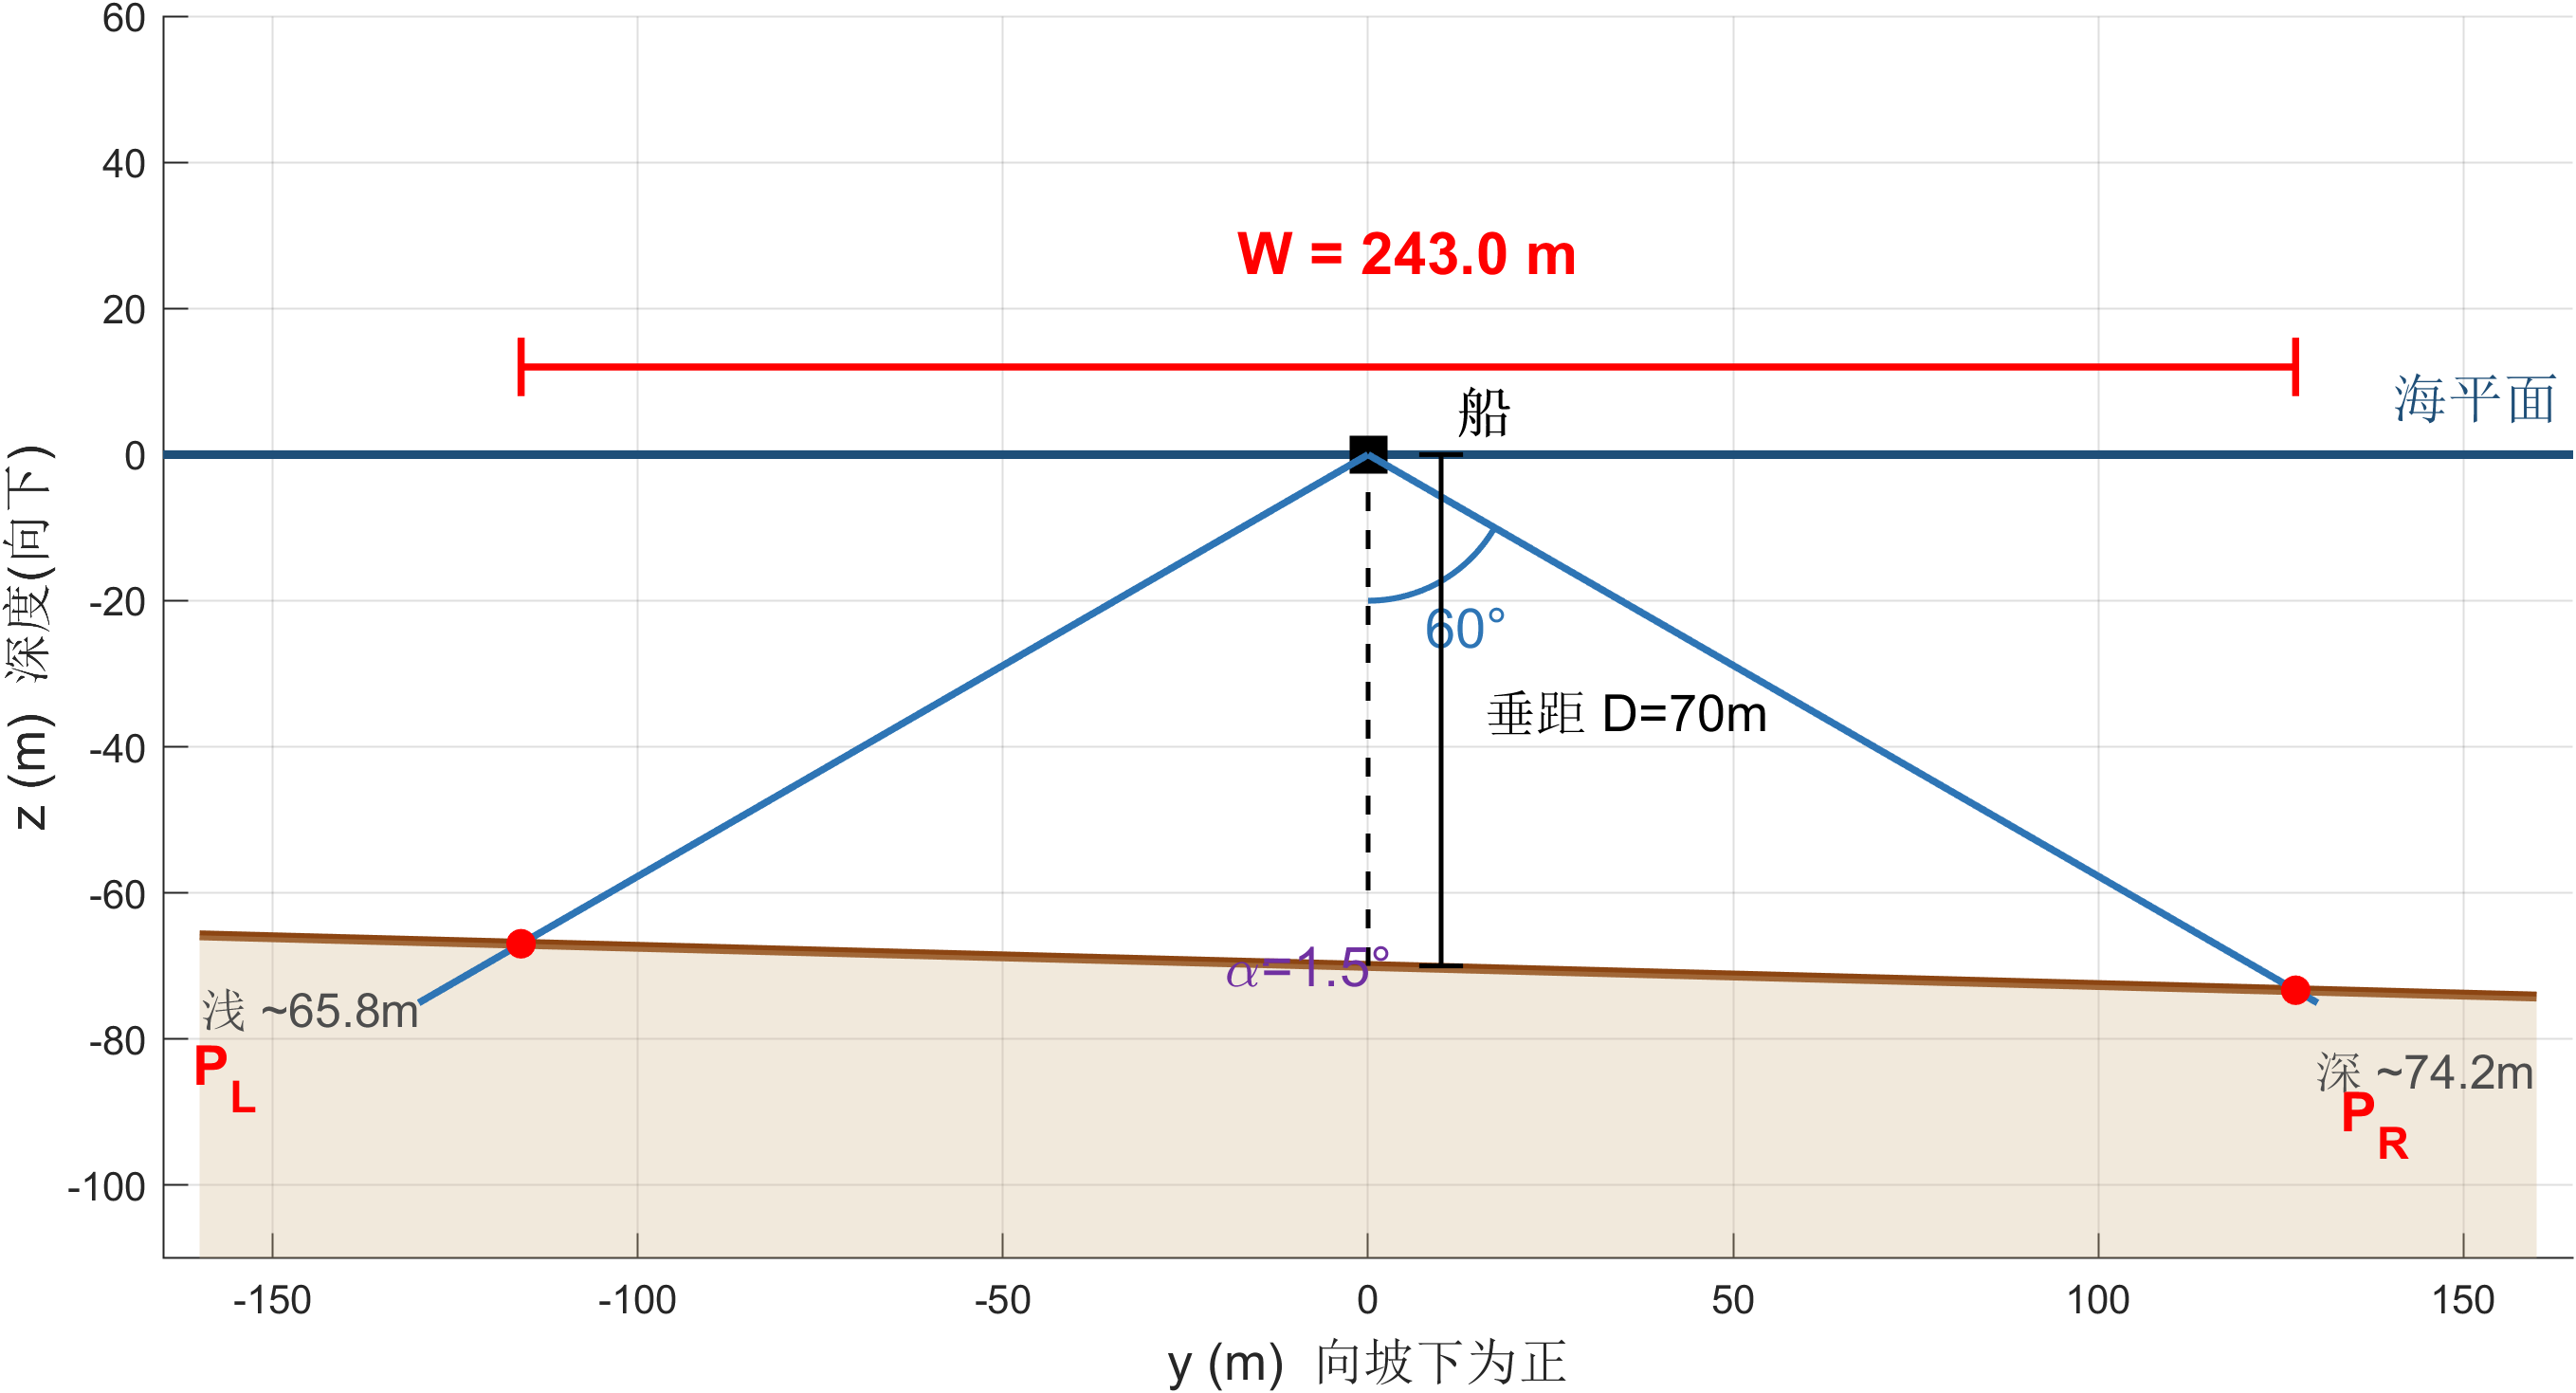
\includegraphics[width=0.75\textwidth]{../fig/fig_q1_geometry.png}
\caption{问题一截面几何示意（半开角 60°、坡度 $\alpha$、覆盖宽度 $W$）}
\label{fig:q1-geo}
\end{figure}


\textbf{2. 重叠率模型}

设相邻两条测线的覆盖宽度分别为 $W_{i-1}$、$W_i$（$W_i\le W_{i-1}$），间距为 $d$。
相邻条带重叠宽度为 $\frac{W_{i-1}}{2}+\frac{W_i}{2}-d$，
以较窄（瓶颈）条带宽度归一化，定义重叠率：
\begin{equation}
    \eta_i = 1 - \frac{d}{W_{\min}}, \qquad W_{\min}=\min(W_{i-1}, W_i)=W_i
    \label{eq:eta}
\end{equation}
该口径与后续问题的重叠率约束设计保持一致：当 $d=0.9W_{\min}$ 时 $\eta=10\%$，
当 $d=W_{\min}$ 时 $\eta=0$（恰好无重叠），$\eta<0$ 表示出现覆盖空隙。

\textbf{3. 测线位置与水深}

测线沿等深线方向（垂直坡面走向）布设，各测线距中心点距离 $x\in\{-800,\ldots,800\}$m，
间距 200m。取 $x$ 正方向为坡上（浅侧），则测线处水深为：
\begin{equation}
    D(x) = D_0 - x\tan\alpha, \qquad D_0 = 70\text{m}
\end{equation}

\subsubsection{求解方法}

求解过程分三步：

\textbf{步骤一：计算宽度系数。}将 $\alpha=1.5^\circ$（$\tan\alpha=0.026186$）代入式 (\ref{eq:width})，
宽度系数为
$K = \frac{1}{\tan30^\circ+\tan\alpha}+\frac{1}{\tan30^\circ-\tan\alpha} = 3.47124$，
即覆盖宽度与水深成正比，$W = K\cdot D$。系数中两项分别对应左右波束：
$\frac{1}{\tan30^\circ+\tan\alpha}=1.65690$（向坡上一侧，坡面抬升使波束更早与坡面相交），
$\frac{1}{\tan30^\circ-\tan\alpha}=1.81434$（向坡下一侧，坡面下沉使交点更远），
两侧不对称正是坡度 $\alpha$ 造成覆盖中心偏离测线正下方的原因。

\textbf{步骤二：计算各测线水深与覆盖宽度。}由 $D(x)=70-x\tan\alpha$ 计算 9 条测线水深，
再由 $W=KD$ 得到覆盖宽度。计算中采用统一的网格精度（0.01m）以保证
各位置数据可比，避免四舍五入的累积误差。

\textbf{步骤三：计算重叠率并判定空隙。}按式 (\ref{eq:eta}) 计算相邻条带重叠率，
并判断是否出现空隙（$\eta<0$）。重叠率的分母取相邻两条中较浅者的宽度
（瓶颈准则），与后续问题的约束设计保持同一口径。

\subsubsection{结果分析}

9 条测线的水深、覆盖宽度与重叠率计算结果如表~1~所示：

\begin{table}[htbp]
\centering
\caption{问题一计算结果（间距 $d=200$m）}
\label{tab:q1}
\begin{adjustbox}{width=\textwidth}
\begin{tabular}{cccccccccc}
\toprule[1.5pt]
距中心点距离/m & -800 & -600 & -400 & -200 & 0 & 200 & 400 & 600 & 800 \\ \midrule[1pt]
海水深度/m  & 90.95 & 85.71 & 80.47 & 75.24 & 70.00 & 64.76 & 59.53 & 54.29 & 49.05 \\
覆盖宽度/m  & 315.71 & 297.53 & 279.35 & 261.17 & 242.99 & 224.81 & 206.63 & 188.45 & 170.27 \\
与前一条重叠率 & --- & 32.78\% & 28.40\% & 23.42\% & 17.69\% & 11.03\% & 3.21\% & 空隙 11.55m & 空隙 29.73m \\
\bottomrule[1.5pt]
\end{tabular}
\end{adjustbox}
\end{table}

条带俯视覆盖情况如图~\ref{fig:q1-cov} 所示。

\begin{figure}[htbp]
\centering
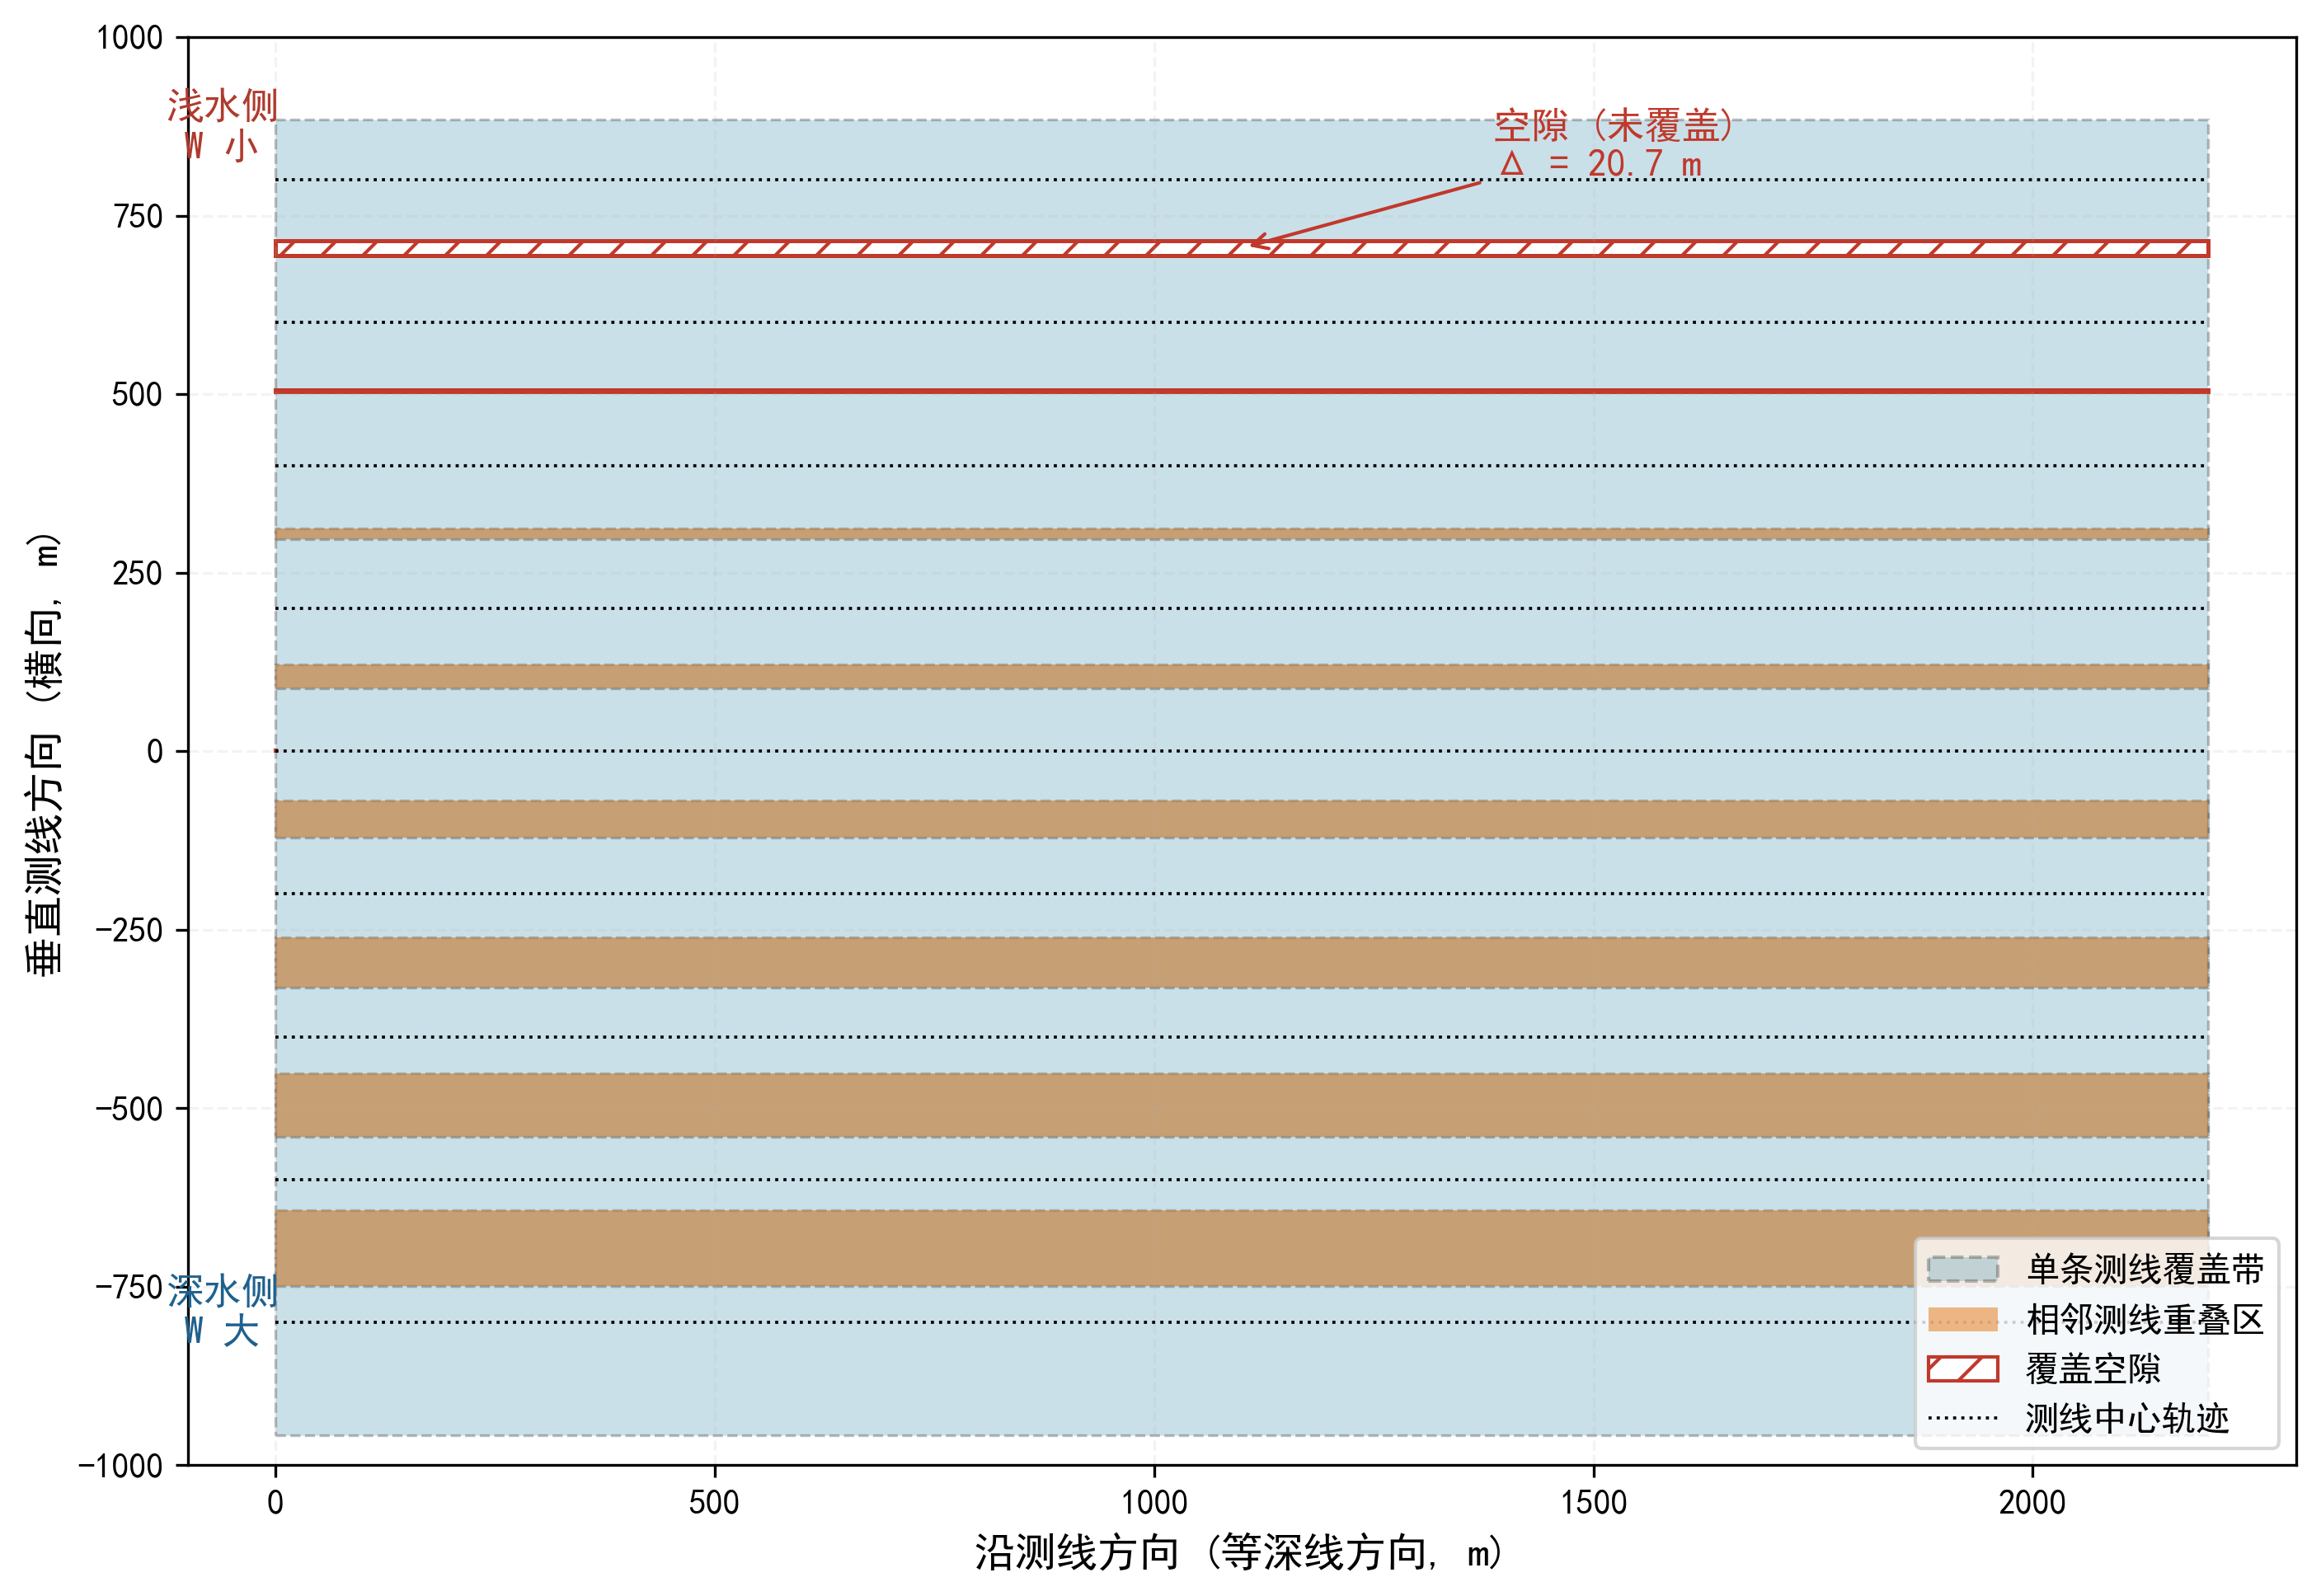
\includegraphics[width=0.95\textwidth]{../fig/fig_q1_coverage_overview.png}
\caption{问题一条带覆盖俯视图（条带随水深收窄，浅水区出现空隙）}
\label{fig:q1-cov}
\end{figure}


结果表明：

（1）覆盖宽度随水深线性递减，自深水侧 315.71m 单调降至浅水侧 170.27m，
递减率即为 $K\tan\alpha\approx0.09$ m/m；
（2）重叠率按瓶颈准则自 32.78\% 单调递减，至 $x=600$m 处 $\eta<0$，
出现 11.55m 空隙，$x=800$m 处空隙扩大至 29.73m；
（3）空隙出现的临界位置由 $W(x)=d$ 反解：$x^* = \frac{D_0-d/K}{\tan\alpha}\approx560$m，
与表~1 中 $x=400$m 处仍有 3.21\% 重叠、$x=600$m 处转为空隙的规律完全吻合。
覆盖宽度与重叠率随测线位置的变化如图~\ref{fig:q1-trend} 所示。

\begin{figure}[htbp]
\centering
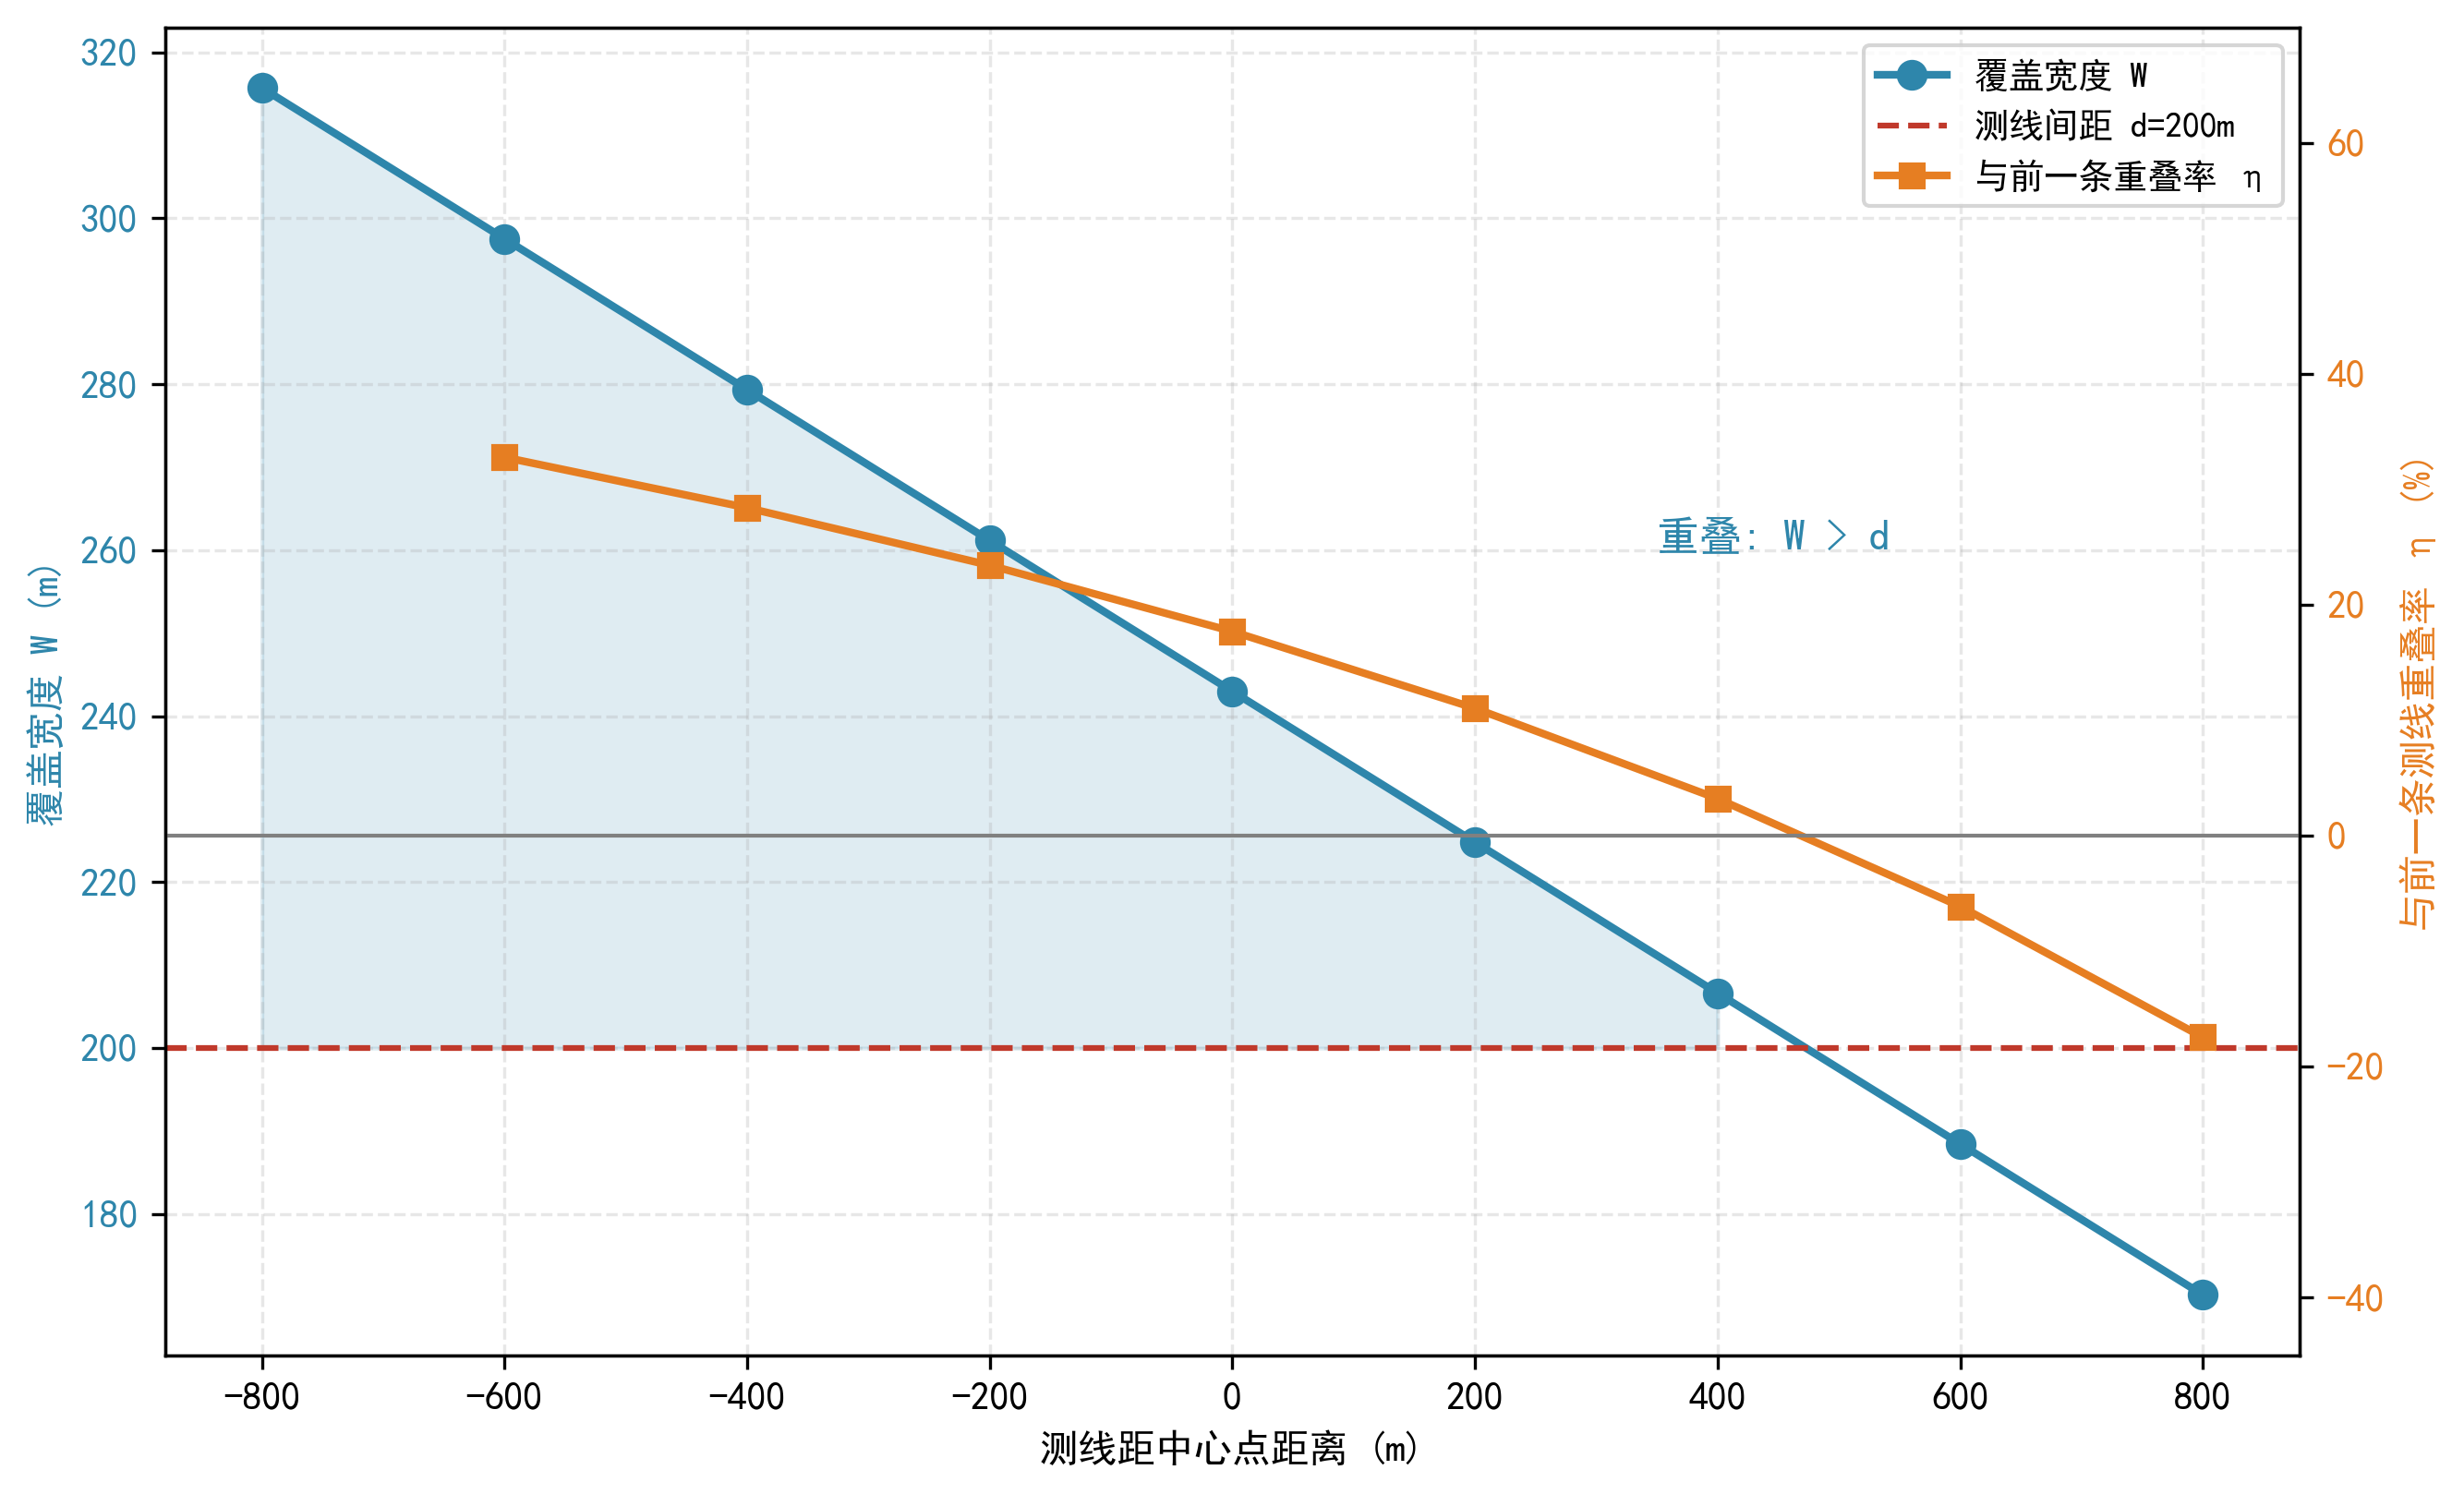
\includegraphics[width=0.85\textwidth]{../fig/fig_q1_trend.png}
\caption{覆盖宽度与重叠率随测线位置的变化（双轴）}
\label{fig:q1-trend}
\end{figure}


固定间距下浅水区条带变窄是覆盖的瓶颈：深水区条带宽、重叠率充足，
浅水区条带收窄后间距相对过大，重叠率先减后转为空隙。

进一步分析各位置的结果：
（1）$x=-800\sim800$m 间水深线性变化 90.95$\to$49.05m，
覆盖宽度同步线性递减，二者比例恒为宽度系数 $K=3.47124$，
验证了 $W\propto D$ 的线性关系；
（2）重叠率自 32.78\% 起每 200m 约下降 5 个百分点，递减近似匀速
（$x=400$m 处仍有 3.21\% 的正重叠），至 $x=600$m 处跨越零值；
（3）空隙宽度随位置加速扩大：$x=600$m 处 11.55m、$x=800$m 处 29.73m，
空隙增速与宽度递减率一致，空隙区条带已无法覆盖间距的一半以上。

上述结果说明，\textbf{固定测线间距无法兼顾深、浅水区的覆盖需求}，
浅水区的重叠率（而非深水区）构成设计的约束瓶颈——
这一结论为问题三的自适应间距设计提供了直接依据：
间距必须随水深（条带宽度）逐条调整，而非固定常数。


\subsection{问题二的建模与求解}

\subsubsection{模型构建}

\textbf{1. 沿测线方向的水深变化}

以 $L$ 表示测线距海域中心点的距离（正方向为坡上），$\beta$ 表示测线与坡面法向
水平投影的夹角。测线方向与坡向的空间夹角导致沿测线方向的水深变化为：
\begin{equation}
    H(L,\beta) = H_0 - L\tan\alpha\cos\beta
\end{equation}
当 $\beta=0^\circ$（测线沿坡向）时水深沿测线变化最快；当 $\beta=90^\circ$
（测线沿等深线）时 $\cos\beta=0$，水深不随 $L$ 变化。

\textbf{2. 视坡角}

问题一假设测线垂直于坡面走向，此时波束截面内的地形坡度恰为真实坡度 $\alpha$。
当测线方向任意时，波束截面（垂直于测线的平面）与坡面的交线不再沿最大坡向，
截面内看到的地形坡度是真实坡度在测线法线方向的投影，称为视坡角 $\alpha'$。
设测线方向与坡面法向水平投影的夹角为 $\beta$，则测线法线方向与最大坡向
的水平夹角为 $90^\circ-\beta$，由方向余弦投影得：
\begin{equation}
    \tan\alpha' = \tan\alpha\cdot|\sin\beta|
\end{equation}
当 $\beta=0^\circ$（测线沿最大坡向，即垂直等深线）时视坡角为 0，
波束截面内海底近似水平；当 $\beta=90^\circ$（测线沿等深线）时视坡角最大，
等于真实坡度 $\alpha$。三维几何关系如图~\ref{fig:q2-geo3d} 所示。

\begin{figure}[htbp]
\centering
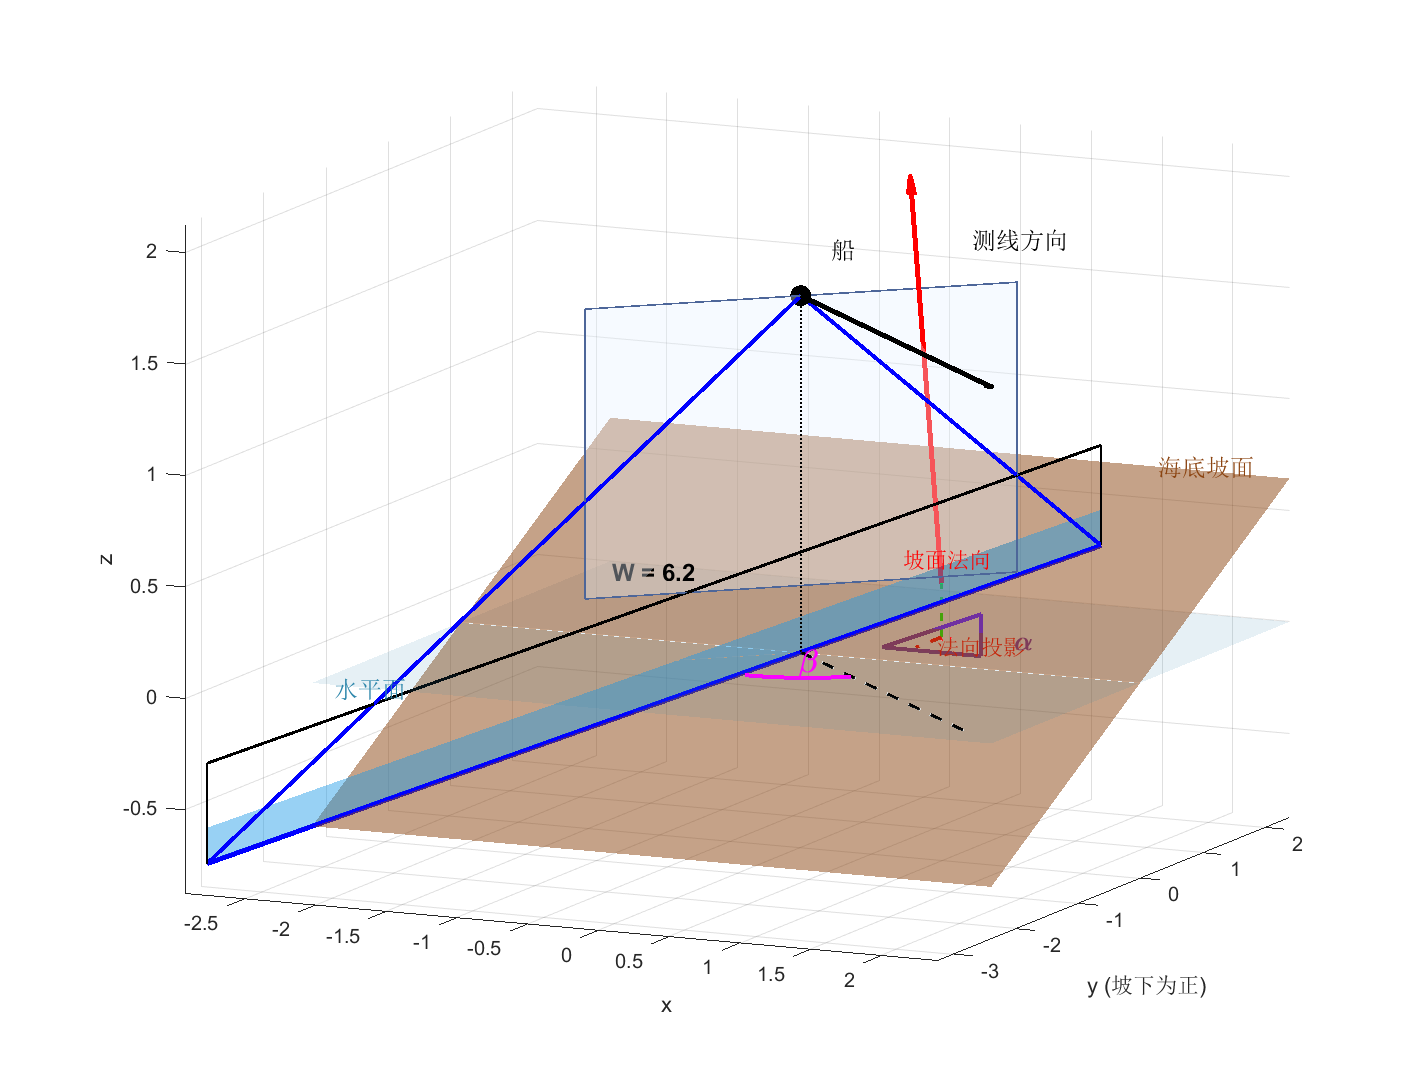
\includegraphics[width=0.8\textwidth]{../fig/fig_q2_geometry3d.png}
\caption{问题二三维几何示意（测线、坡面法向与夹角 $\beta$）}
\label{fig:q2-geo3d}
\end{figure}


\textbf{3. 覆盖宽度公式}

将 $H(L,\beta)$ 与 $\alpha'$ 代入式 (\ref{eq:width})（以视坡角替代真实坡角），得：
\begin{equation}
    \boxed{W(L,\beta) = H(L,\beta)
    \left[\frac{1}{\tan30^\circ+\tan\alpha'} + \frac{1}{\tan30^\circ-\tan\alpha'}\right]}
    \label{eq:W-L-beta}
\end{equation}
该式统一了问题一与问题二：问题一为 $\beta=90^\circ$、$L=0$ 的特例。

\subsubsection{求解方法}

计算流程分三步：

\textbf{步骤一：参数网格设置。}取 $H_0=120$m、$\alpha=1.5^\circ$；
距离参数 $L\in\{0,0.3,\ldots,2.1\}$（海里，步长 0.3 海里，共 8 个位置），
方向参数 $\beta\in\{0^\circ,45^\circ,\ldots,315^\circ\}$（步长 45°，共 8 个方向），
构成 $8\times8$ 的参数网格。

\textbf{步骤二：逐点计算。}对网格中每一组 $(L,\beta)$：
先由 $\cos\beta$ 求该处水深 $H(L,\beta)$，再由 $|\sin\beta|$ 求视坡角 $\alpha'$，
最后代入式 (\ref{eq:W-L-beta}) 得覆盖宽度 $W(L,\beta)$。
计算采用统一精度（0.1m），并利用 $H_0=120$m 的对称性
（$\beta$ 与 $180^\circ-\beta$ 结果相同）作为交叉校验。

\textbf{步骤三：结果组织与校验。}将 8 个方向的宽度按 $\beta$ 升序排列成表，
并校验三个性质：对称性（$\beta\leftrightarrow180^\circ-\beta$）、
单调性（$W$ 随 $L$ 的变化方向）、以及 $\beta=90^\circ/270^\circ$ 行的恒定性。

\subsubsection{结果分析}

$8\times8$ 覆盖宽度表（单位 m）如表~2~所示：

\begin{table}[H]
\centering
\caption{覆盖宽度 $W(L,\beta)$（单位：m）}
\label{tab:q2}
\small
\begin{adjustbox}{max width=\textwidth}
\begin{tabular}{ccccccccc}
\toprule[1.5pt]
$\beta\backslash L$（海里） & 0.0 & 0.3 & 0.6 & 0.9 & 1.2 & 1.5 & 1.8 & 2.1 \\ \midrule[1pt]
$0^\circ$   & 415.7 & 365.3 & 314.9 & 264.5 & 214.1 & 163.7 & 113.3 & 62.9 \\
$45^\circ$  & 416.1 & 380.5 & 344.8 & 309.1 & 273.4 & 237.8 & 202.1 & 166.4 \\
$90^\circ$  & 416.6 & 416.6 & 416.6 & 416.6 & 416.6 & 416.6 & 416.6 & 416.6 \\
$135^\circ$ & 416.1 & 451.8 & 487.5 & 523.1 & 558.8 & 594.5 & 630.2 & 665.8 \\
$180^\circ$ & 415.7 & 466.1 & 516.5 & 566.9 & 617.3 & 667.7 & 718.1 & 768.5 \\
$225^\circ$ & 416.1 & 451.8 & 487.5 & 523.1 & 558.8 & 594.5 & 630.2 & 665.8 \\
$270^\circ$ & 416.6 & 416.6 & 416.6 & 416.6 & 416.6 & 416.6 & 416.6 & 416.6 \\
$315^\circ$ & 416.1 & 380.5 & 344.8 & 309.1 & 273.4 & 237.8 & 202.1 & 166.4 \\
\bottomrule[1.5pt]
\end{tabular}
\end{adjustbox}
\end{table}

$W(L,\beta)$ 的曲面与热力分布如图~\ref{fig:q2-combined} 所示。

\begin{figure}[htbp]
\centering
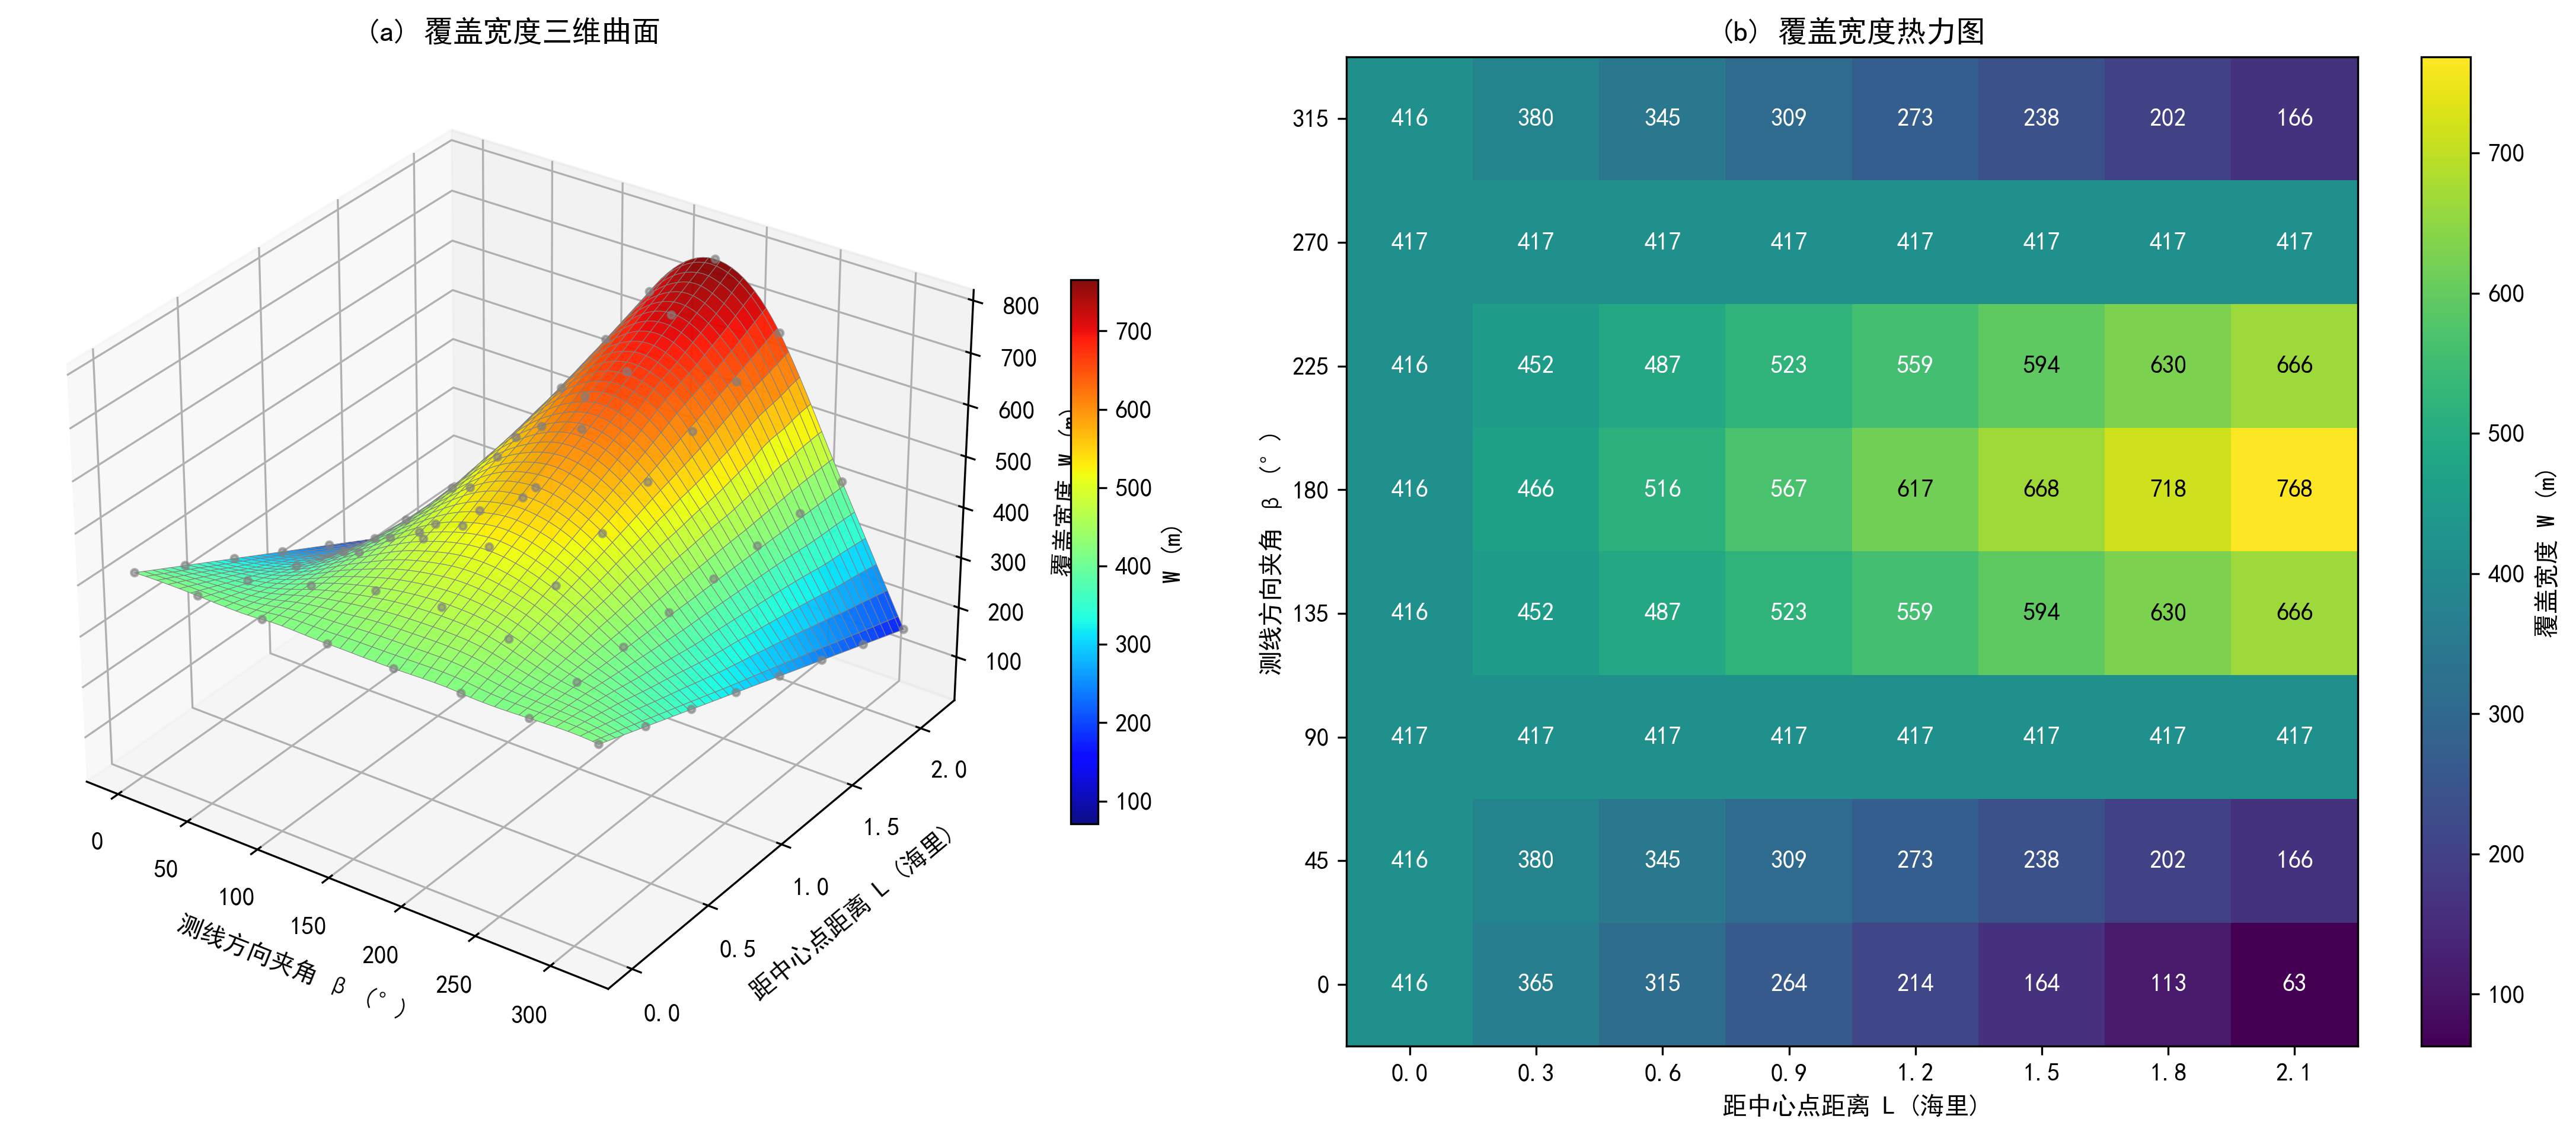
\includegraphics[width=0.95\textwidth]{../fig/fig_q2_combined.png}
\caption{覆盖宽度 $W(L,\beta)$ 三维曲面与热力图}
\label{fig:q2-combined}
\end{figure}


由表~2 可得三个关键性质：

（1）\textbf{对称性}：$\beta$ 与 $180^\circ-\beta$ 的结果相同（测线无方向），
$45^\circ$ 与 $135^\circ$、$225^\circ$ 与 $315^\circ$ 各行数值一致，验证了公式的对称结构
（$\cos\beta$ 与 $|\sin\beta|$ 均关于 $\beta=90^\circ$ 对称）；

（2）\textbf{单调性}：$\beta=0^\circ$ 时 $W$ 随 $L$ 递减最快
（$L$ 正方向为坡上，水深减小，从 415.7m 降至 62.9m）；
$\beta=180^\circ$ 时递增（向深水方向，增至 768.5m）；
$\beta=45^\circ$ 时变化放缓（166.4m），反映水深变化率 $\propto\cos\beta$ 的衰减；

（3）\textbf{特殊性}：$\beta=90^\circ,270^\circ$（沿等深线）时 $W$ 恒为 416.6m，
不随 $L$ 变化且为该行最大值。机理：测线沿等深线时沿线水深不变，
波束截面内的视坡角恒为最大坡度 $\alpha$，条带宽度恒定且最大；
而其他方向的水深沿线变化导致宽度不均匀，且视坡角减小使宽度略有下降。

性质（3）具有重要的工程意义：\textbf{测线沿等深线方向布设时，
条带宽度在整个测线长度上保持恒定且最大}，既简化了间距设计
（间距可按常数条带宽度确定），又使覆盖效率最高。

进一步从表中提取定量信息：
（1）宽度范围 62.9$\sim$768.5m，跨度为 12 倍——测线方向与位置
对覆盖宽度的影响十分显著，测线设计不可忽略方向维度的选择；
（2）$\beta=0^\circ$ 行每 0.3 海里宽度下降约 50m（线性递减），
$\beta=180^\circ$ 行对称递增，两者递减率相同（约 167m/海里），
由 $H(L,\beta)$ 的线性结构与宽度公式的线性性共同决定；
（3）$L=0$ 列（中心点）各方向宽度差异小于 0.9m（415.7$\sim$416.6m），
说明中心点附近视坡角对宽度的影响可忽略，方向差异主要
由水深变化路径的不同所致——这是"方向优化的收益来自覆盖几何
而非单点宽度"的直观体现，与问题四的分析相呼应。

综上，问题二为测线方向选择提供了量化依据：\textbf{测线沿等深线
（$\beta=90^\circ$）时条带宽度恒定最大，应作为问题三测线方向的
首选，并通过方向扫描定量验证}。不同测线方向的 $W(L)$ 剖面族如图~\ref{fig:q2-profile} 所示。

\begin{figure}[htbp]
\centering
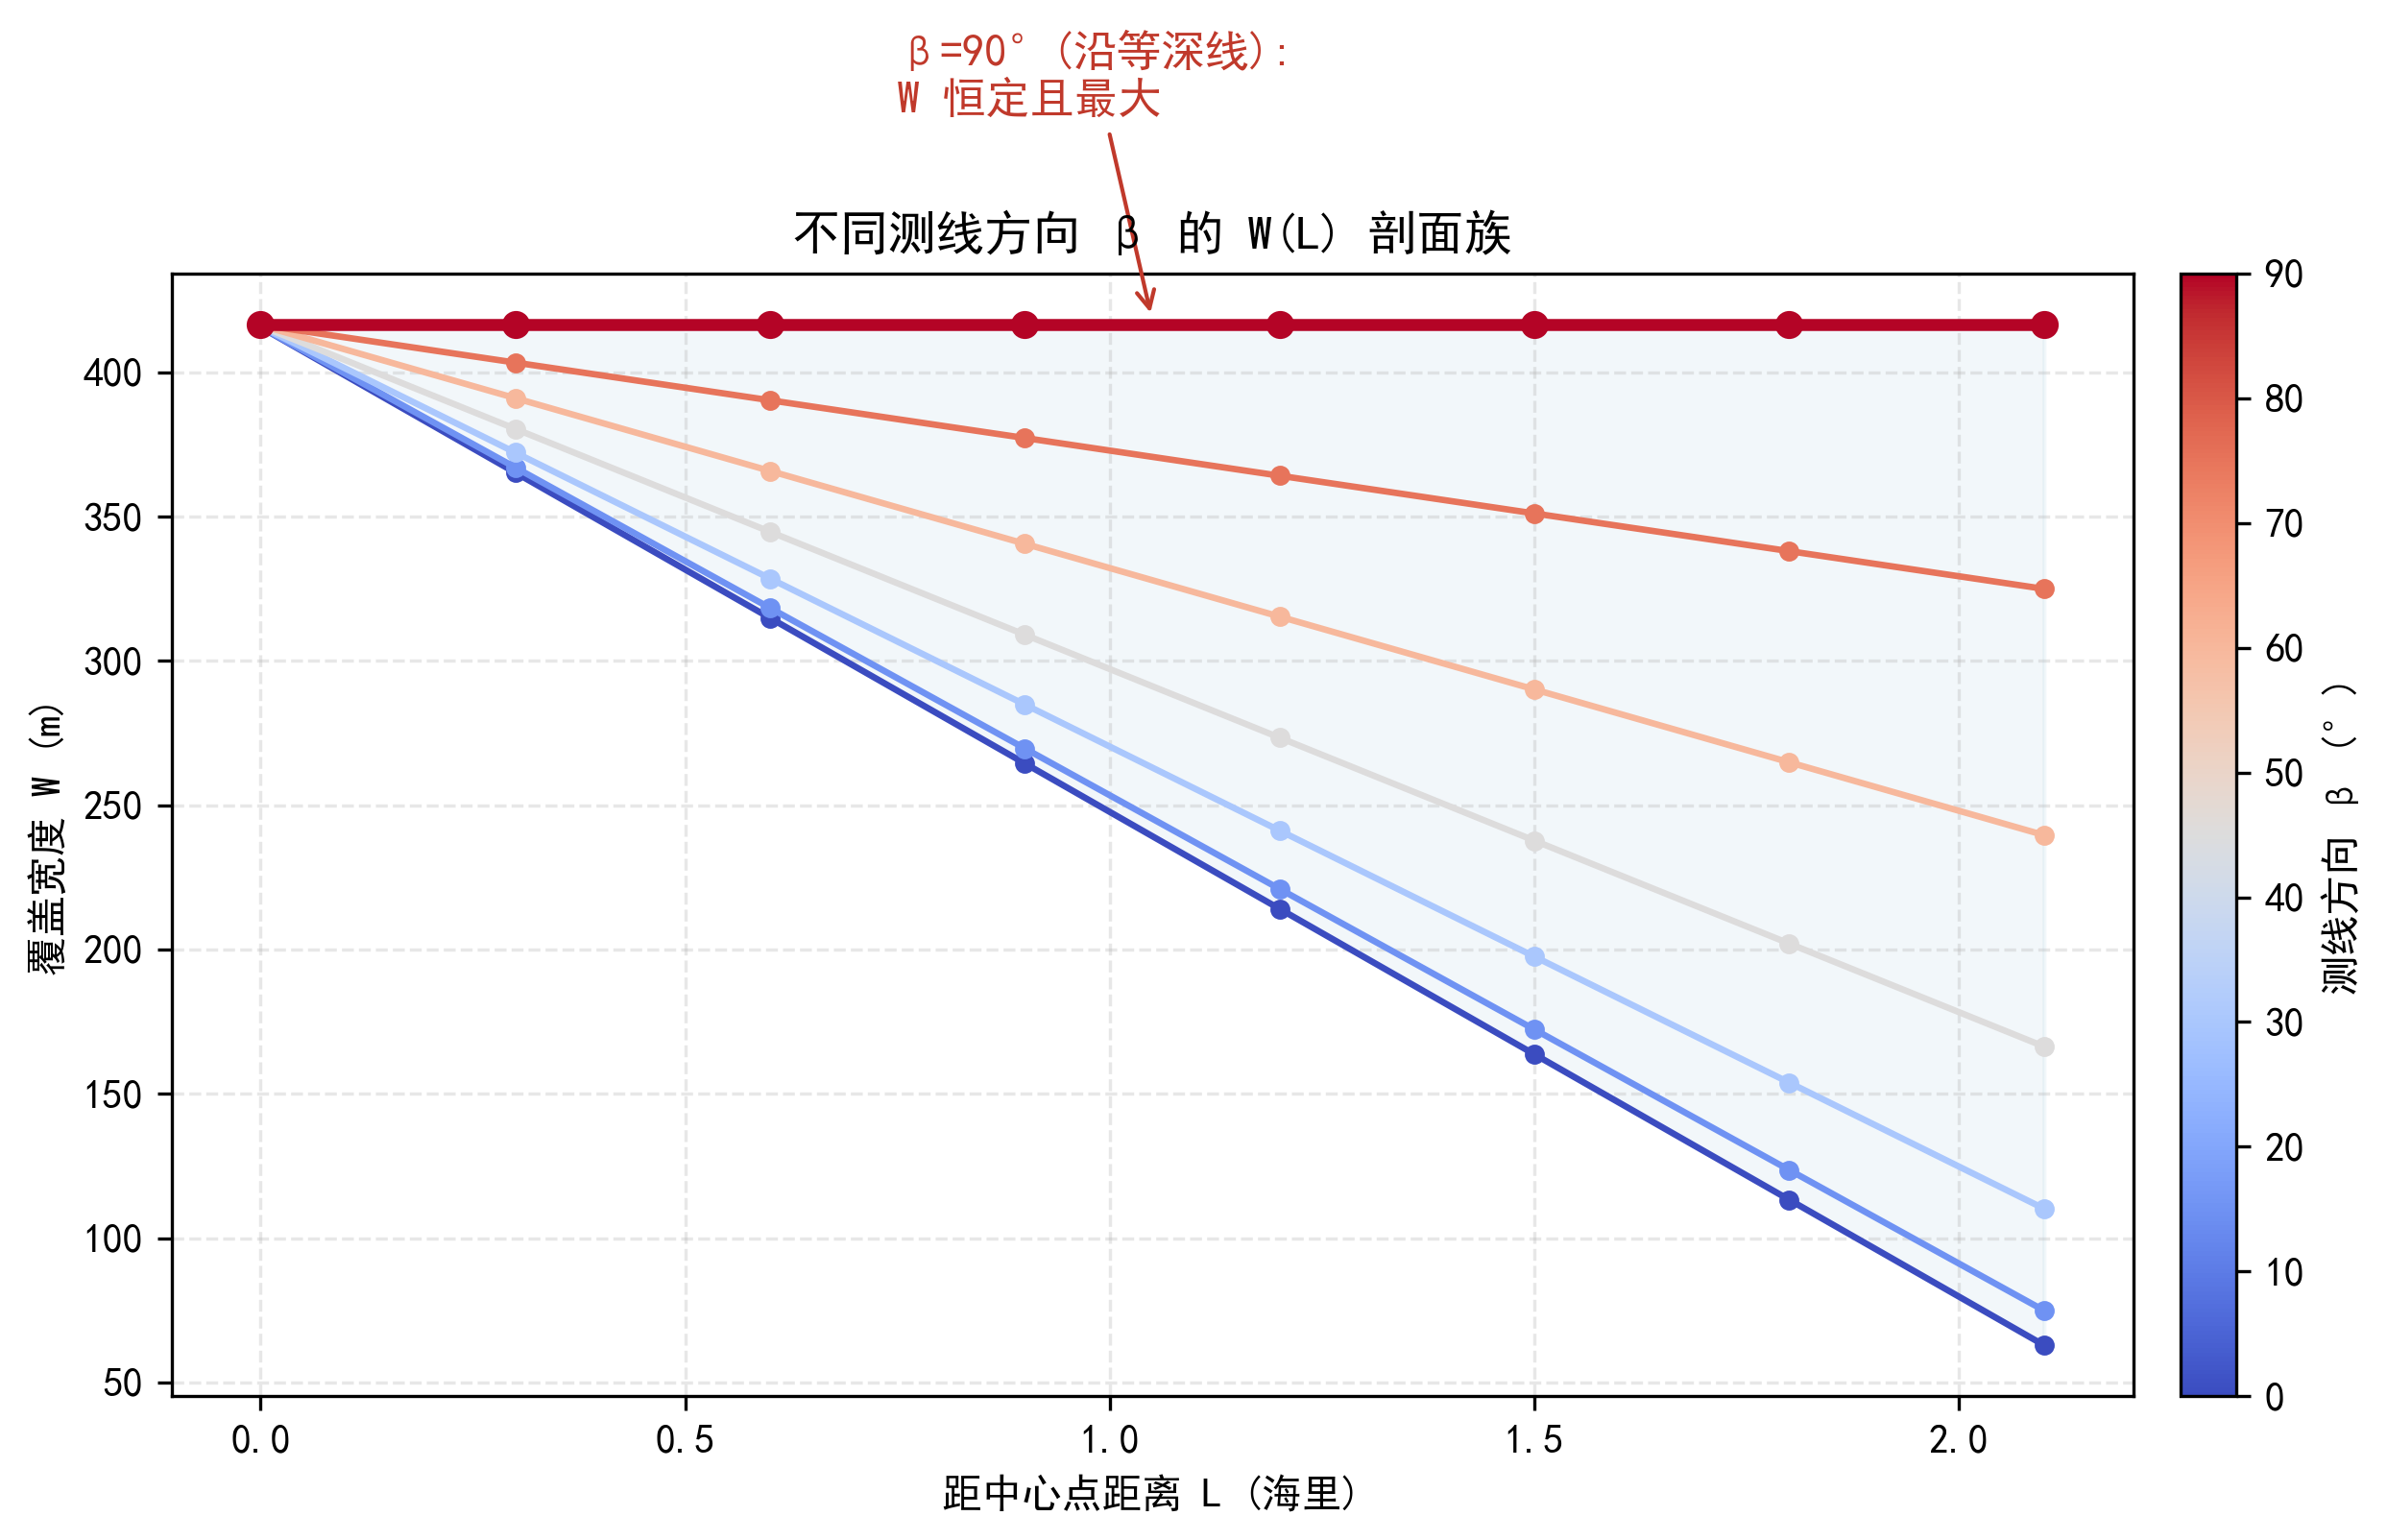
\includegraphics[width=0.8\textwidth]{../fig/fig_q2_profile.png}
\caption{不同测线方向的 $W(L)$ 剖面族（$\beta=90^\circ$ 恒定最大）}
\label{fig:q2-profile}
\end{figure}



\subsection{问题三的建模与求解}

\subsubsection{模型构建}

\textbf{1. 测线方向优化模型}

海域为南北 2 海里、东西 4 海里的矩形，中心水深 110m，西深东浅，坡度 $\alpha=1.5^\circ$。
测线贯穿南北、单线长 2 海里固定，故总长最短等价于条数最少。

由问题二性质（3），测线沿等深线（南北向，$\beta=90^\circ$）时条带宽度恒定最大，
理论上应为最优方向。但最优性需定量验证：测线方向改变后，
测线长度（斜穿海域的截线长度）、条带宽度（视坡角变化）与间距
（瓶颈宽度变化）三者同时改变，无法由解析直接比较。
为此建立\textbf{方向扫描模型}：以测线方向角 $\beta$ 为决策参数，
对每个 $\beta$ 构造平行测线族——测线族沿法线方向逐条推进，
间距由重叠率约束逐条确定（见间距递推模型），测线族总长即为
该方向的布设成本 $L(\beta)$，最优方向为 $\beta^*=\arg\min L(\beta)$。

\textbf{2. 间距递推模型}

测线方向确定后，问题转化为沿法线方向确定各测线的间距序列。
由重叠率约束 $10\%\le\eta\le20\%$ 与式 (\ref{eq:eta}) 反解间距：
\begin{equation}
    0.8\,W_{\min} \le d \le 0.9\,W_{\min}
\end{equation}
即间距必须落在相邻两条中较浅者宽度的 $0.8\sim0.9$ 倍之间。
重叠率越大则间距越小、条数越多，故总长最短等价于\textbf{每条间距取允许上限}
$d_i=0.9\,W_{\min}$，此时相邻条带重叠率恰为 10\%，贴着约束下界——这是
"约束越紧、方案越优"思想下的最优策略。

以 $x$ 表示测线东西向位置，$W(x)=K\,[H_0-x\tan\alpha]$ 为宽度函数。
间距递推的完整形式为 $x_{i+1}-x_i = 0.9\,W_{\min}(x_i, x_{i+1})$，
其中瓶颈 $W_{\min}=\min\{W(x_i),W(x_{i+1})\}=W(x_{i+1})$（西深东浅，
下一条位于浅侧、宽度更小）。将 $W(x_{i+1})=K(H_0-x_{i+1}\tan\alpha)$ 代入
并整理为显式递推：
\begin{equation}
    x_{i+1} = \frac{x_i + 0.9\,K\,H_0}{1 + 0.9\,K\,\tan\alpha}
    \label{eq:recur}
\end{equation}
由式 (\ref{eq:recur}) 可见间距 $d_i = x_{i+1}-x_i = 0.9W(x_{i+1})$ 随水深
单调递减，即\textbf{间距自深水端向浅水端逐条收窄}，与浅水区条带变窄的物理规律一致。

\textbf{3. 起点的对称性}

间距递推的收敛性不依赖起点方向：间距序列由宽度场唯一决定，
深水端起步与浅水端起步正反向递推相互对称，条数相同。

\subsubsection{求解方法}

\textbf{步骤一：方向扫描。}对 $\beta\in[0^\circ,180^\circ]$ 每 $15^\circ$ 一次，
以同一口径模拟布设——测线族沿法线方向推进、深水端起步、
间距 $d=0.9W_{\min}$（$W_{\min}$ 取该测线浅端宽度），
统计各方向的测线总长（因 $\beta$ 与 $180^\circ-\beta$ 对称，仅列出 $0\sim90^\circ$）。

\textbf{步骤二：间距递推。}初始测线由"覆盖西边界"确定：
$x_1 - W(x_1)/2 = X_W$，解得 $x_1 = (X_W + KH_0/2)/(1+K\tan\alpha/2)$；
随后按式 (\ref{eq:recur}) 逐条递推，终止条件为
$x_{i+1}+W(x_{i+1})/2\ge X_E$（最后一条覆盖东边界）。
同时从东边界反向递推验证条数一致（起点对称性）。
取深水端为布设起点：工程上优先测量深水区可及早获取风险较高的
深水地形资料，且深水区条带宽、间距大，前期测线数少、效率高。

\textbf{步骤三：航迹计算。}蛇形折返连接相邻测线，第 $i$ 段转弯弧为
半径 $r_i=d_i/2$ 的半圆弧，转弯航程 $L_{\text{turn}}=\sum_i \pi r_i$；
保守口径取 $r_i=\max(d_i/2,\,200\text{m})$（船最小转弯半径限制）。

\textbf{步骤四：多算法验证。}
（1）\textbf{动态规划}——以 5m 为网格对测线位置离散化，
状态为测线位置，转移代价为该间距段的覆盖代价，搜索全局最小条数方案；
（2）\textbf{遗传算法}——以测线条数 $N$ 为决策变量、间距序列为基因，
适应度函数惩罚覆盖缺口与重叠率越界，种群采用贪心初始化
（由间距递推序列扰动生成）；
（3）\textbf{K-means 分区}——测线位置按横坐标聚类为 $K$ 区，
区内统一间距（区平均宽度 $\times0.9$），区界处以重叠条带衔接。

\subsubsection{结果分析}

\textbf{1. 方向扫描结果}

方向扫描的相对总长如表~3 所示：

\begin{table}[htbp]
\centering
\caption{测线总长随方向角 $\beta$ 的扫描结果（相对值，$\beta=90^\circ$ 为 1.00）}
\label{tab:q3-beta}
\begin{adjustbox}{max width=\textwidth}
\begin{tabular}{cccccccc}
\toprule[1.5pt]
$\beta$（度） & 0 & 15 & 30 & 45 & 60 & 75 & 90 \\ \midrule[1pt]
相对总长 & 5.69 & 4.50 & 3.22 & 2.32 & 1.77 & 1.37 & 1.00 \\
\bottomrule[1.5pt]
\end{tabular}
\end{adjustbox}
\end{table}

扫描结果表明：总长随 $\beta$ 单调递减，$\beta=90^\circ$（南北向，沿等深线）时最短，
$\beta=0^\circ$（东西向，垂直等深线）时为最短值的 5.69 倍。
机理：测线沿等深线时沿线水深恒定、条带宽度最大且恒定，布设效率最高；
垂直等深线时测线沿坡向横穿整个深度带，条带宽度随水深急剧变化、
测线也更长（东西向截线长 4 海里，而南北向仅 2 海里）。
$0^\circ\sim90^\circ$ 之间为两者的连续过渡，总长单调递减。
扫描曲线如图~\ref{fig:q3-beta} 所示。

\begin{figure}[htbp]
\centering
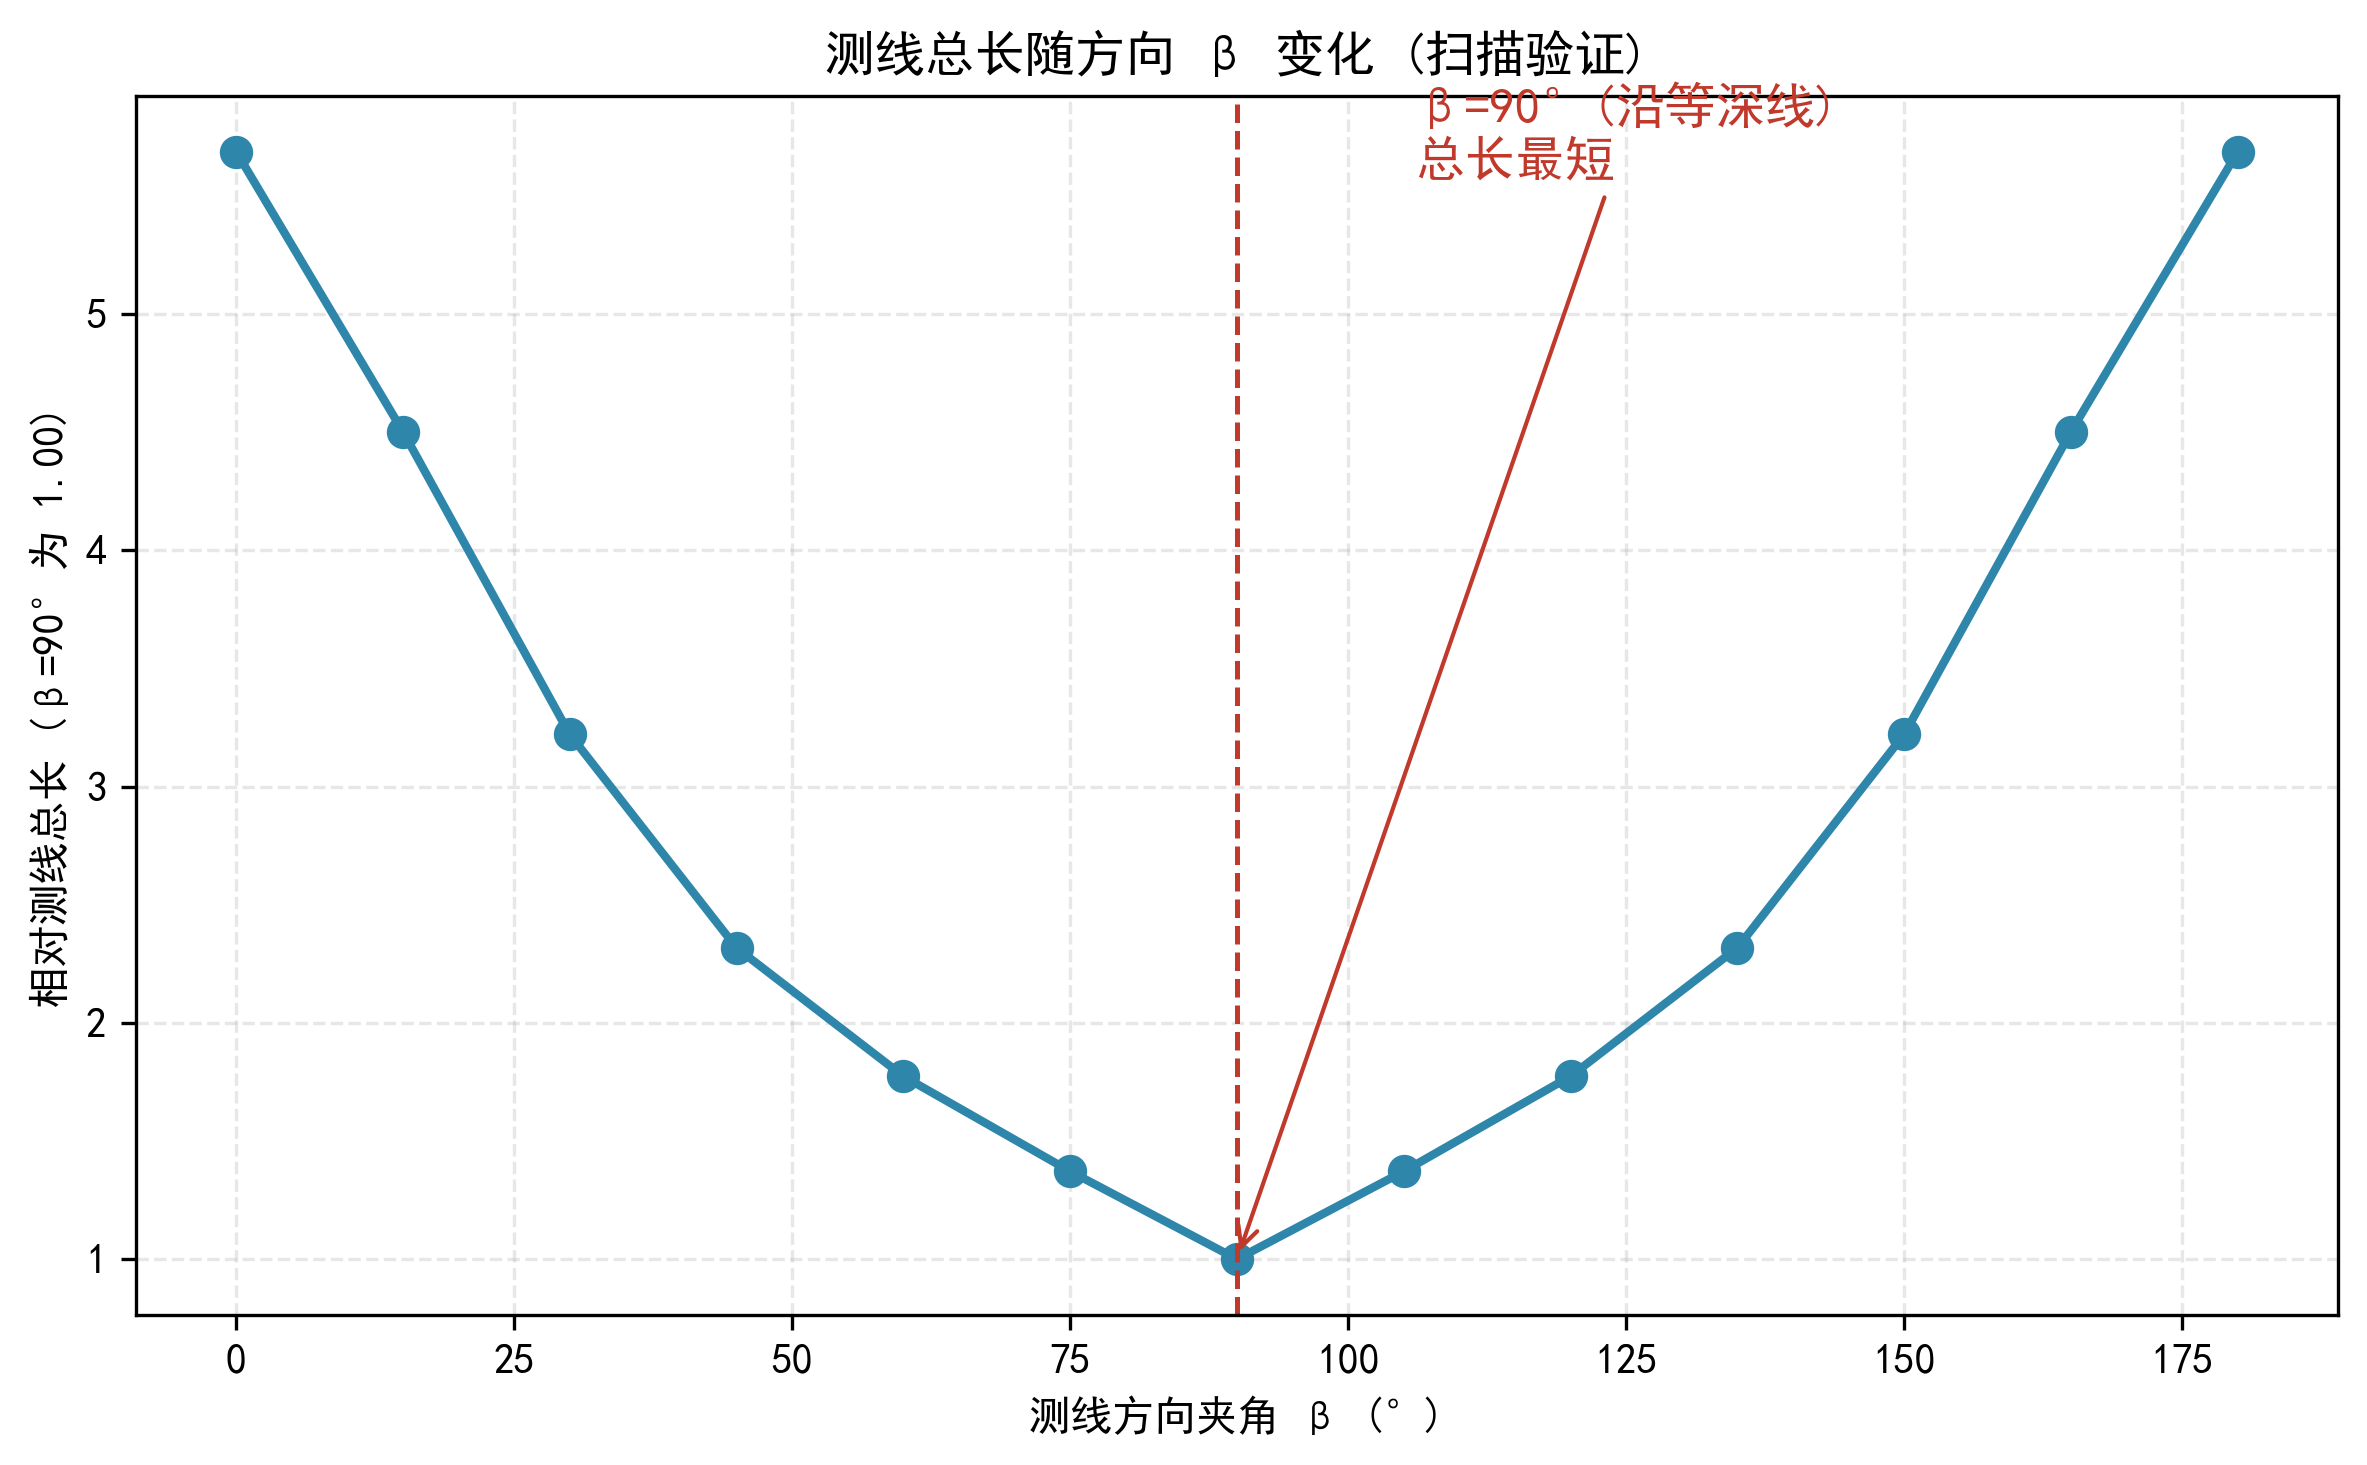
\includegraphics[width=0.8\textwidth]{../fig/fig_q3_beta_scan.png}
\caption{测线总长随方向角的扫描曲线（$\beta$ 与 $180^\circ-\beta$ 等价）}
\label{fig:q3-beta}
\end{figure}


\textbf{2. 布设方案结果}

按式 (\ref{eq:recur}) 递推得 36 条南北向测线，总长 $36\times2=72$ 海里，
相邻条带重叠率全部恰为 10\%（贴着约束下界，方案最经济）；
间距自深水端 571.8m 单调递减至浅水端 39.5m；
全覆盖验证通过（西边界覆盖至 $-3704.0$m $\le X_W=-3704$m，
东边界覆盖至 $3740.3$m $\ge X_E=3704$m）。
方案的核心特征：36 条测线的间距序列完全由宽度场决定，
深水区间距大、浅水区间距小，条带在浅水端以 39.5m 的最小间距
精确贴合海域边界，全海域无一处漏测、无一处重叠率低于 10\%。
三维布设效果如图~\ref{fig:q3-3d} 所示。

\begin{figure}[htbp]
\centering
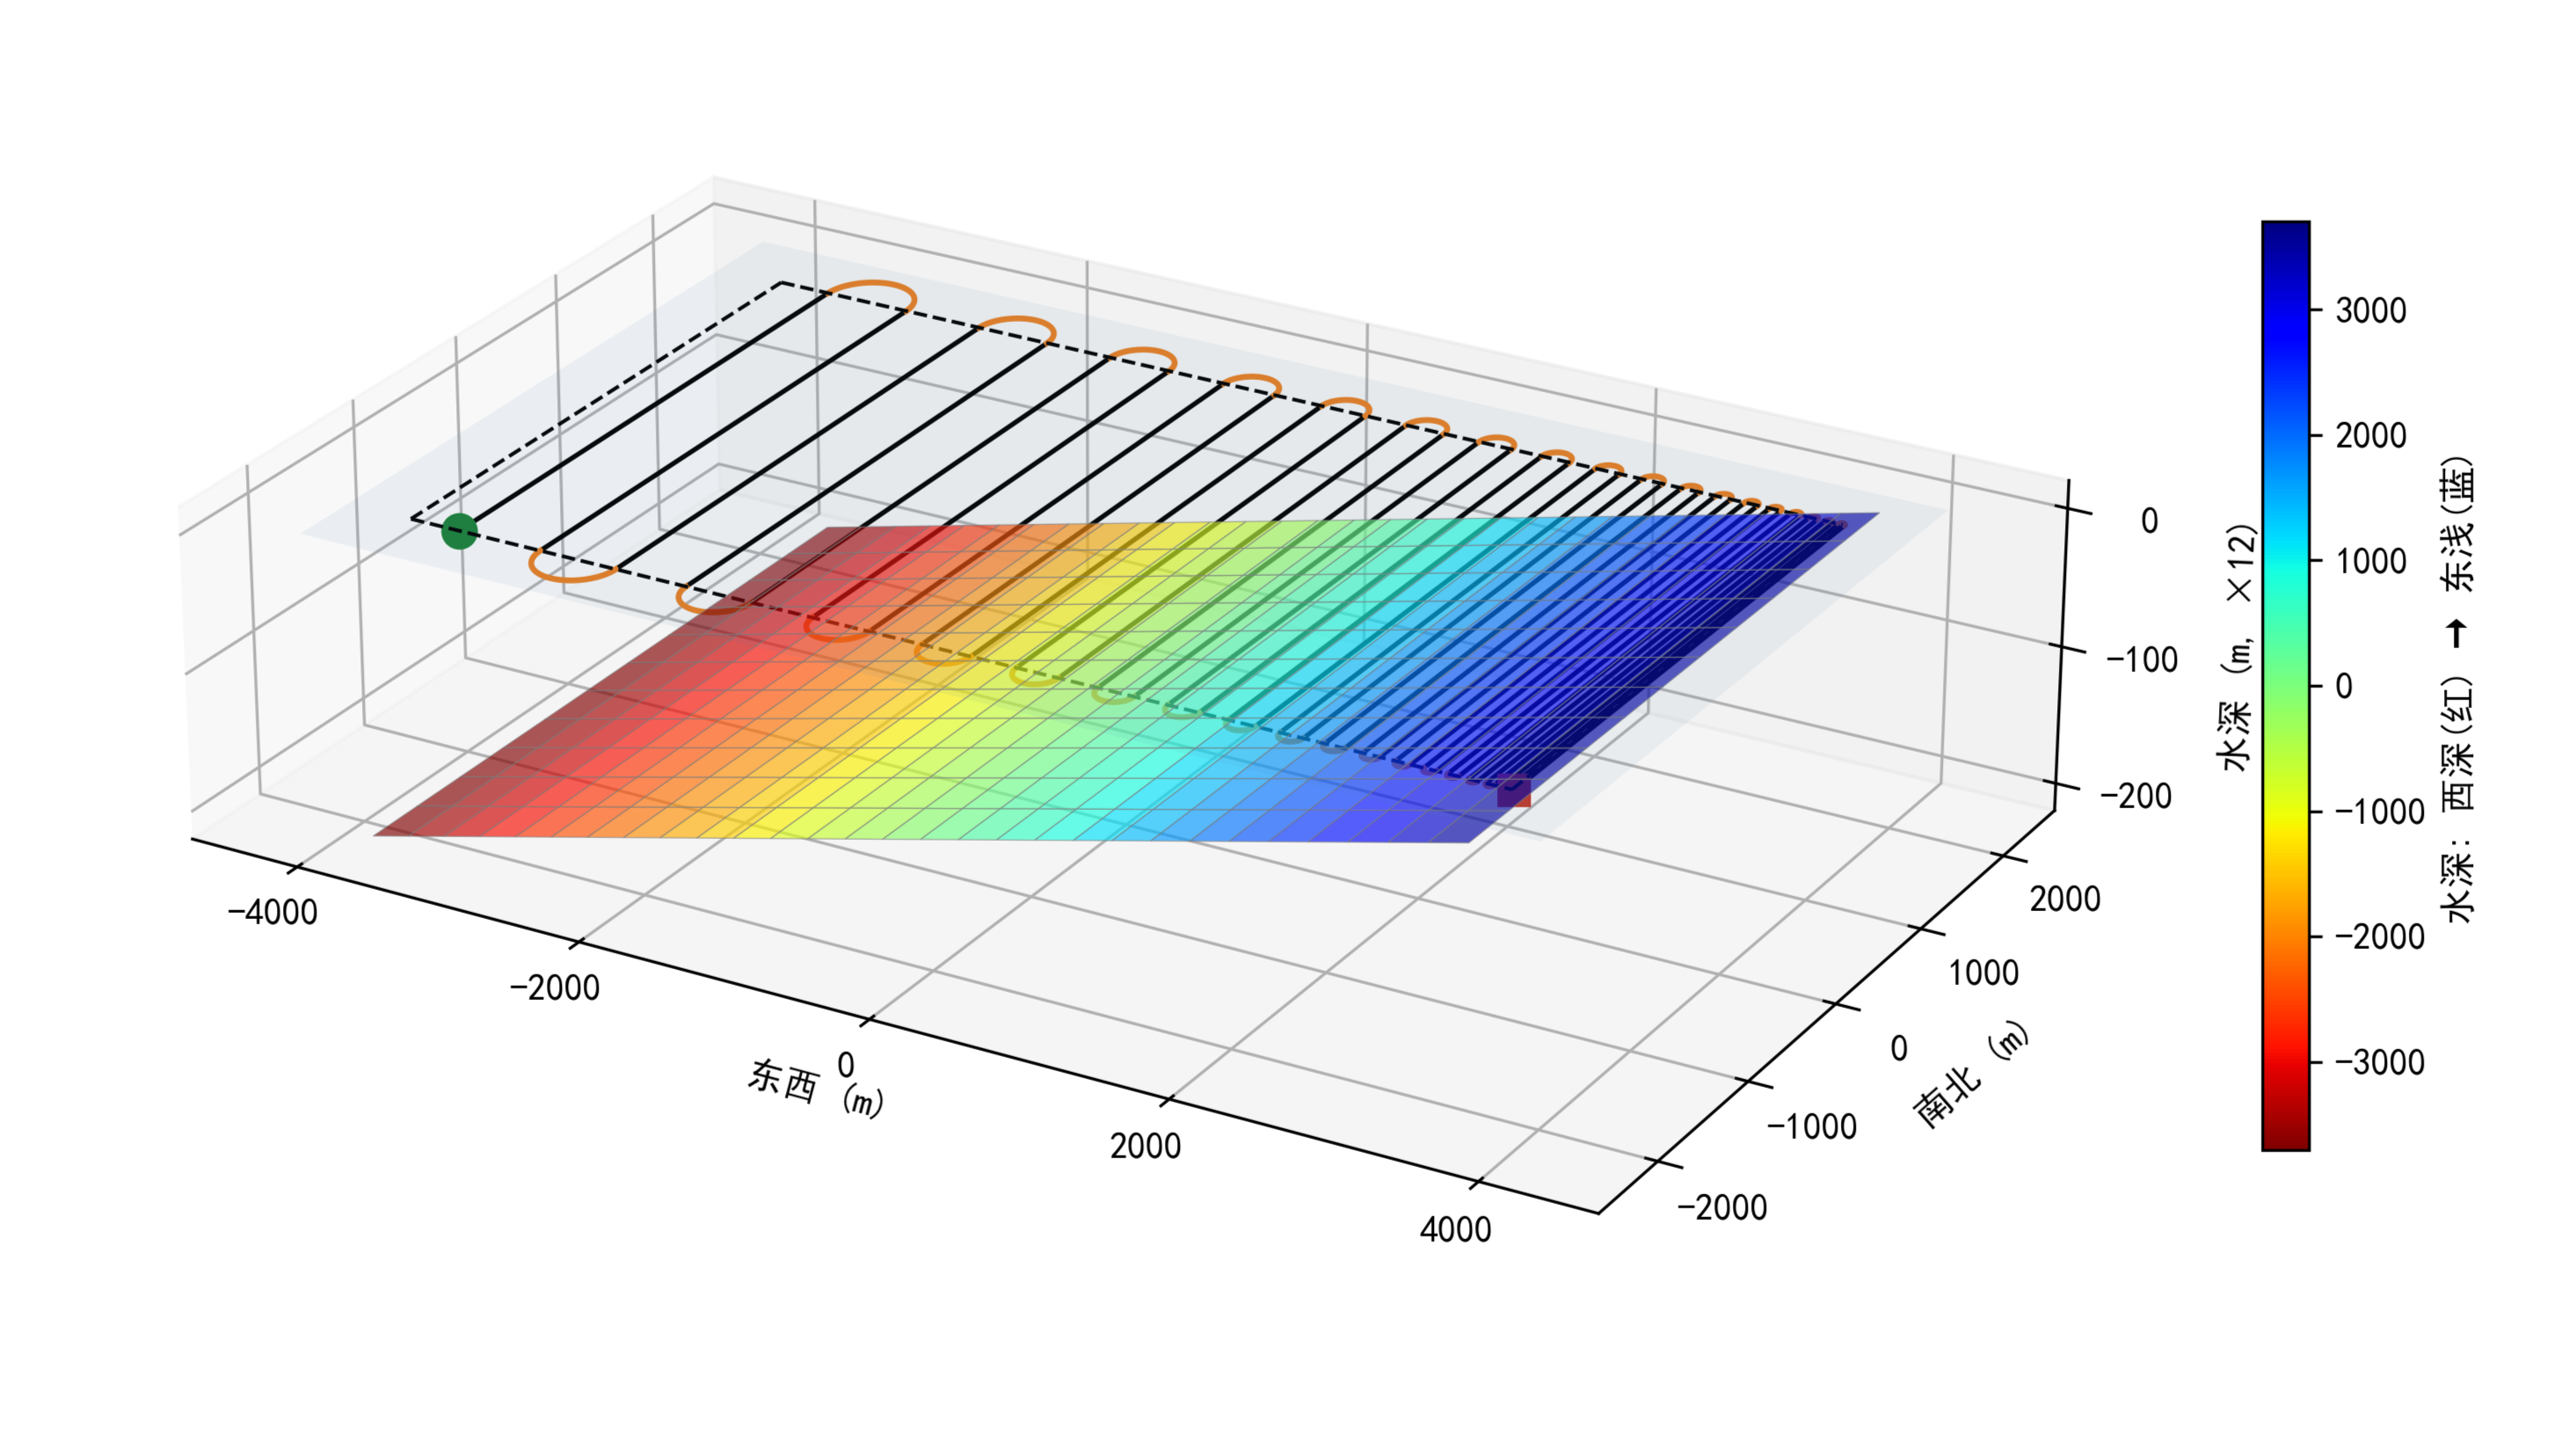
\includegraphics[width=0.95\textwidth]{../fig/fig_q3_3d.png}
\caption{第三问三维布设效果（彩色海底与蛇形航线）}
\label{fig:q3-3d}
\end{figure}


\textbf{3. 航迹分析结果}

测线长度 72 海里不含连接段，实际航行还需计入转弯段。
船以蛇形折返连接相邻测线，35 段折返弧（最小半径 $r=d/2$）转弯航程约 6.00 海里，
完整航迹约 78.0 海里（较测线总长增加 7.7\%）；
若考虑船最小转弯半径 200m，转弯航程增至 12.26 海里，完整航迹 84.3 海里（+14.5\%）。
对比梳形连接（每条测线返回同端出发），其完整航迹达 145.8 海里，近乎翻倍——
\textbf{蛇形折返是连接段最短方案}。转弯段为不可避免的航迹成本，不计入测线总长。
完整测量航迹如图~\ref{fig:q3-track} 所示。

\begin{figure}[htbp]
\centering
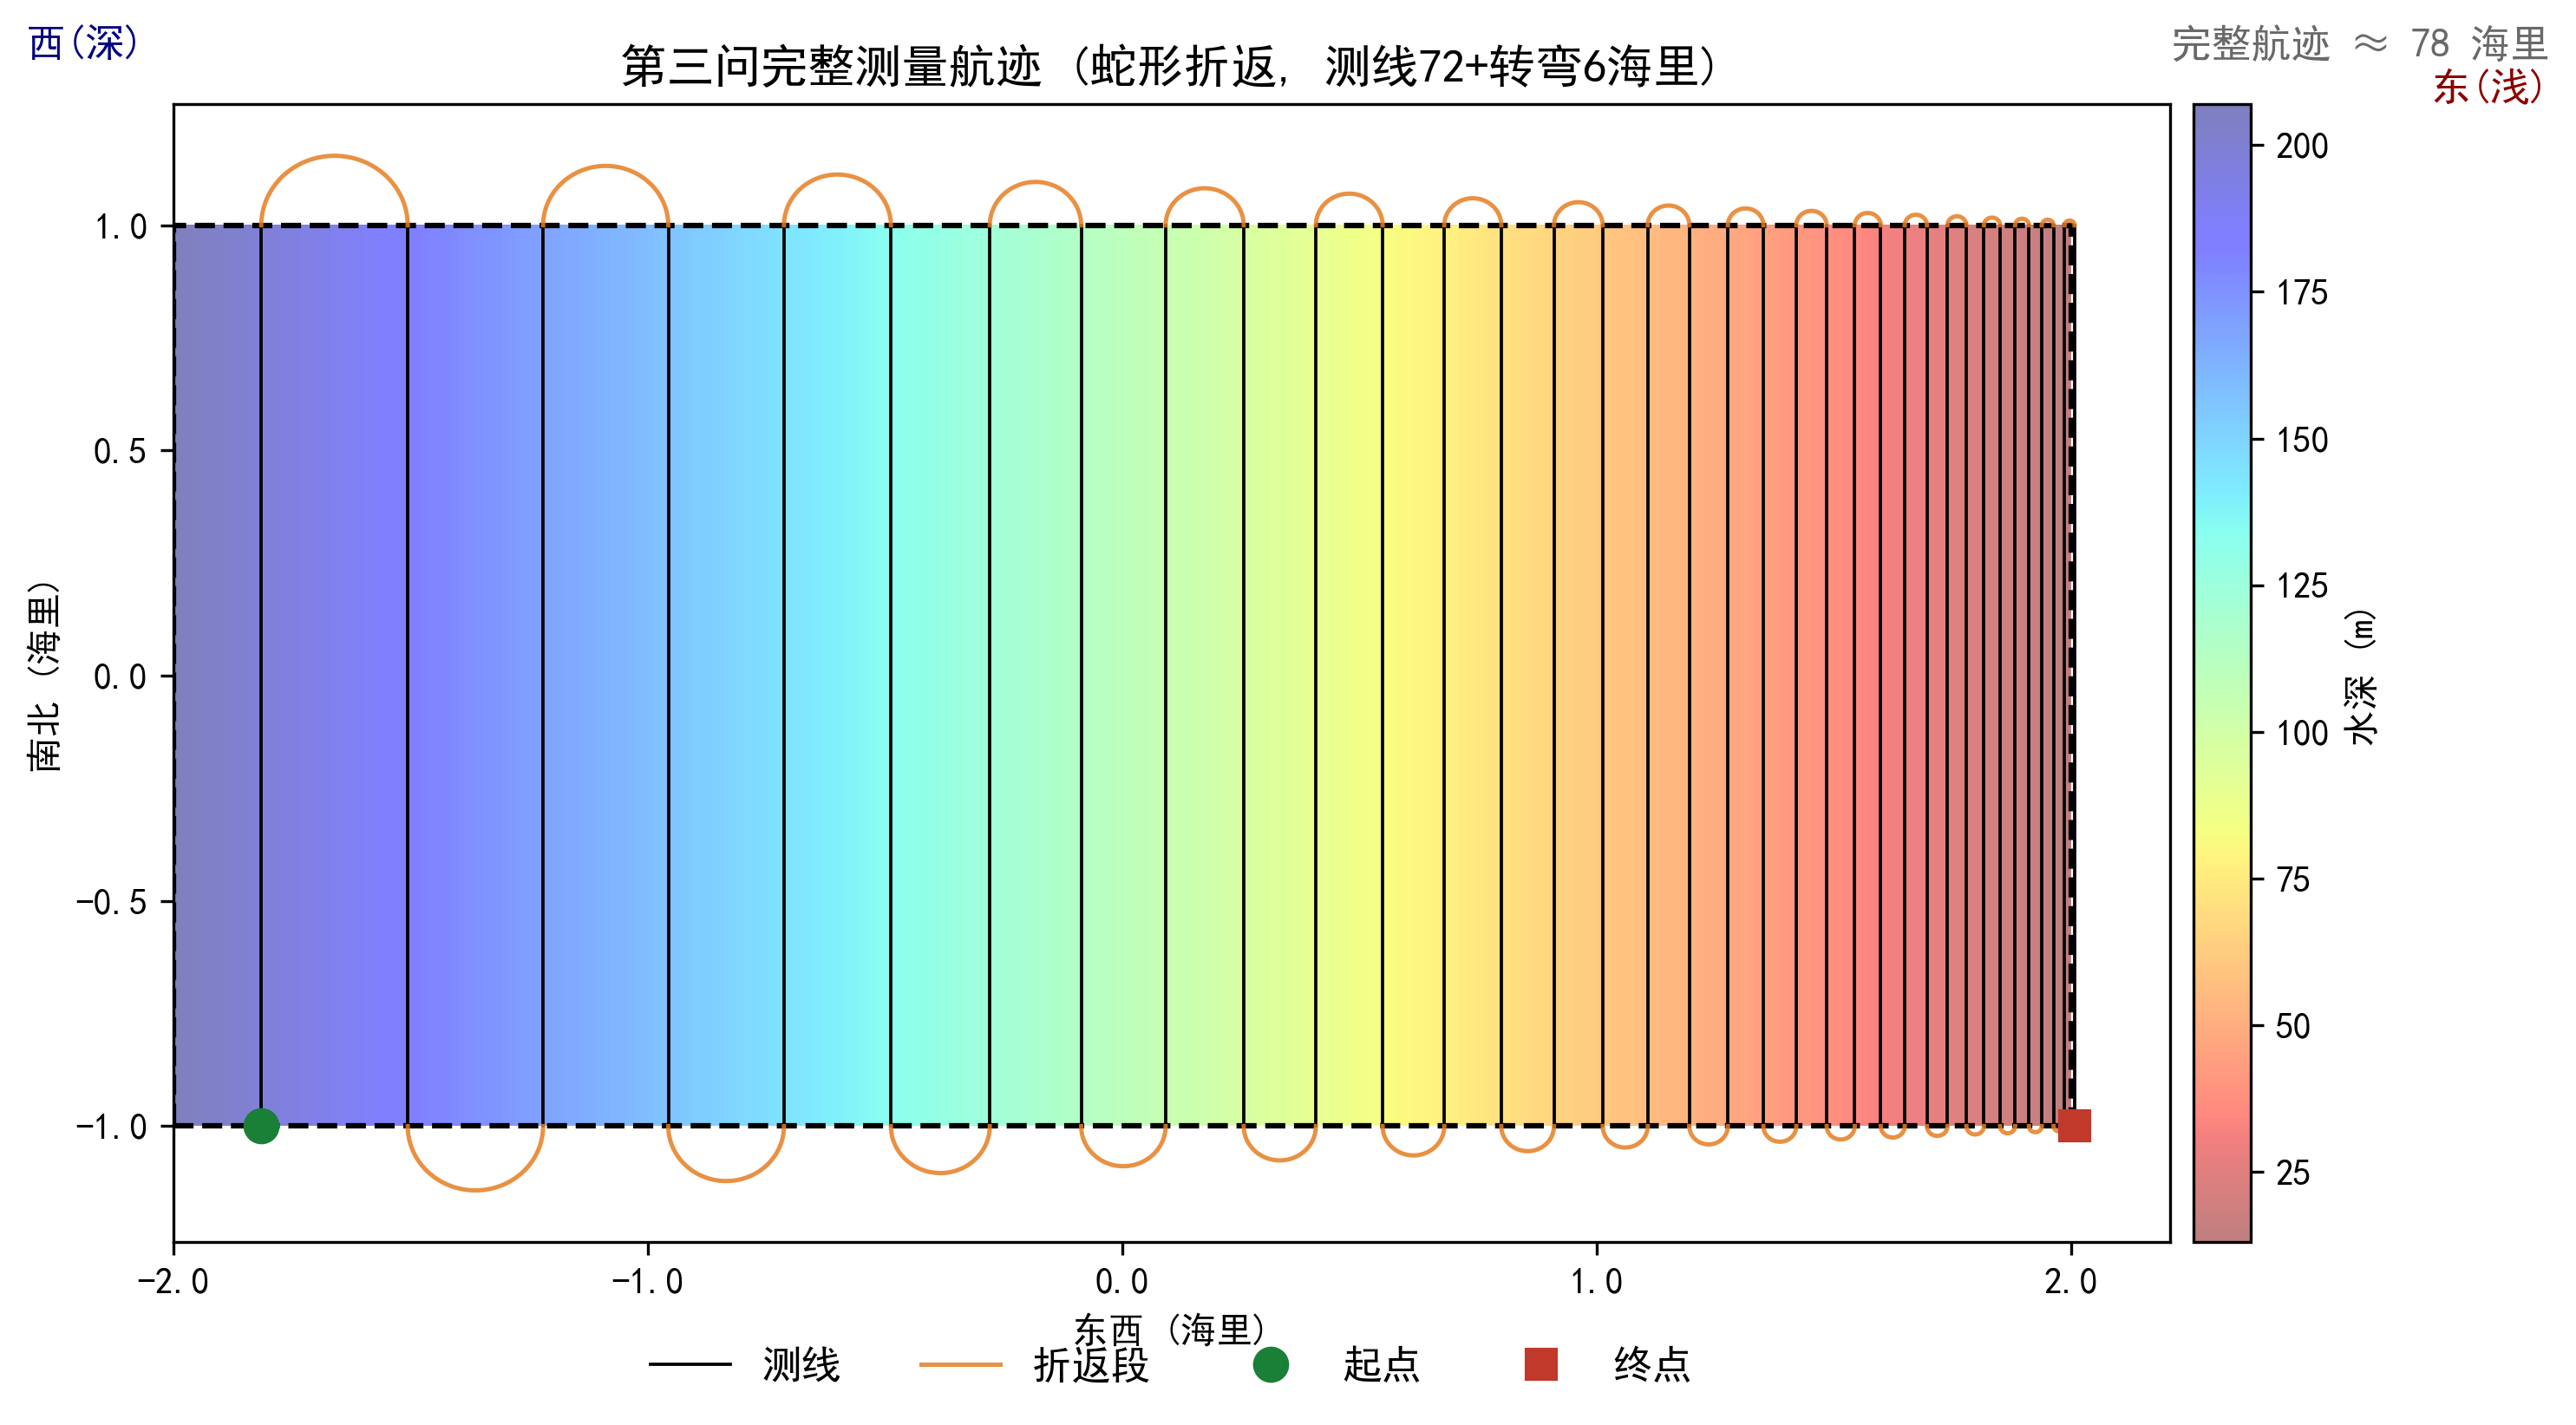
\includegraphics[width=0.95\textwidth]{../fig/fig_q3_track.png}
\caption{第三问完整测量航迹（蛇形折返，测线 72 海里 + 转弯约 6 海里）}
\label{fig:q3-track}
\end{figure}


\textbf{4. 多算法验证结果}：

（1）\textbf{动态规划（最优性验证）}——以 5m 为网格对测线位置离散化，
将"最少条数覆盖"建模为最短路径问题：状态为测线位置，转移代价为
覆盖该间距段所需条数，动态规划搜索全局最小条数方案。
结果仍为 36 条，且与式 (\ref{eq:recur}) 的间距递推序列完全一致，
证明贪心递推（每步取间距上限 $d=0.9W_{\min}$）在平面坡上即为
约束下的全局最优——贪心局部最优与全局最优在此问题中重合。

（2）\textbf{遗传算法（可行域检验）}——以测线条数 $N$ 为决策变量、
间距序列为基因，适应度函数惩罚覆盖缺口与重叠率越界。
关键设计是\textbf{贪心初始化}：初始种群由间距递推序列的扰动生成；
验证 $N=36$ 可行、$N=34/35$ 不可行，与 DP 结论一致。
对照实验表明：纯随机初始化的 GA 无法收敛（可行域过窄——
间距须逐条落在 $[0.8W_{\min},0.9W_{\min}]$ 内，随机序列几乎必然越界），
贪心初始化是 GA 在此类强约束问题中可用的必要前提。

（3）\textbf{K-means 分区近似（对照实验）}——将测线位置按横坐标
聚类为 $K$ 个区（$K=2\sim4$），区内采用统一间距（区平均宽度 $\times0.9$），
区界处以重叠条带衔接。由于区内深度跨度大、条带宽度差异明显
（单区宽度可差 2$\sim$3 倍），统一间距无法兼顾区内深浅两侧，
方案条数达 104$\sim$70 条（$K=2\sim4$），远多于逐条递推的 36 条，
且重叠率波动剧烈。该对照实验说明：\textbf{测线间距必须逐条自适应，
分区平均化处理会显著劣化方案}。

\subsection{问题四的建模与求解}

\subsubsection{数据与地形分析}

附件数据为南北 5 海里、东西 4 海里的单波束测深网格：251$\times$201 点，
网格间距 0.02 海里（约 37m），深度 24.4$\sim$84.4m。
数据预处理与地形特征提取分三步：

\textbf{步骤一：网格化与深度场。}以附件网格点为节点建立水深场 $H(x,y)$，
网格间距近似均匀（37m）；深度范围 24.4$\sim$84.4m，无缺失值。

\textbf{步骤二：梯度场与等深线方向场。}用中心差分计算水深梯度
$g_x=\partial H/\partial x,\ g_y=\partial H/\partial y$；
等深线方向（梯度方向的垂直方向）为 $\theta_{\text{iso}}=\arctan(g_y/g_x)+\pi/2$。
统计结果表明：等深线方向均值 88.4°、\textbf{标准差高达 50.6°}，
等深线严重蜿蜒。

\textbf{步骤三：地形类型判定。}沿东西方向深度自 41m 单调增至 118m
（平均坡度仅 0.83°，坡度缓），而南北方向存在 56$\sim$79m 的显著起伏，
说明该海域为\textbf{缓坡背景上的丘陵型地形}：整体上西浅东深、
等深线大致南北走向，但局部凹凸使等深线剧烈弯曲。
这一特征决定了第四问不能直接套用第三问"沿等深线直线布设"的结论，
测线方向需通过扫描重新确定。地形特征如图~\ref{fig:q4-terrain} 所示。

\begin{figure}[htbp]
\centering
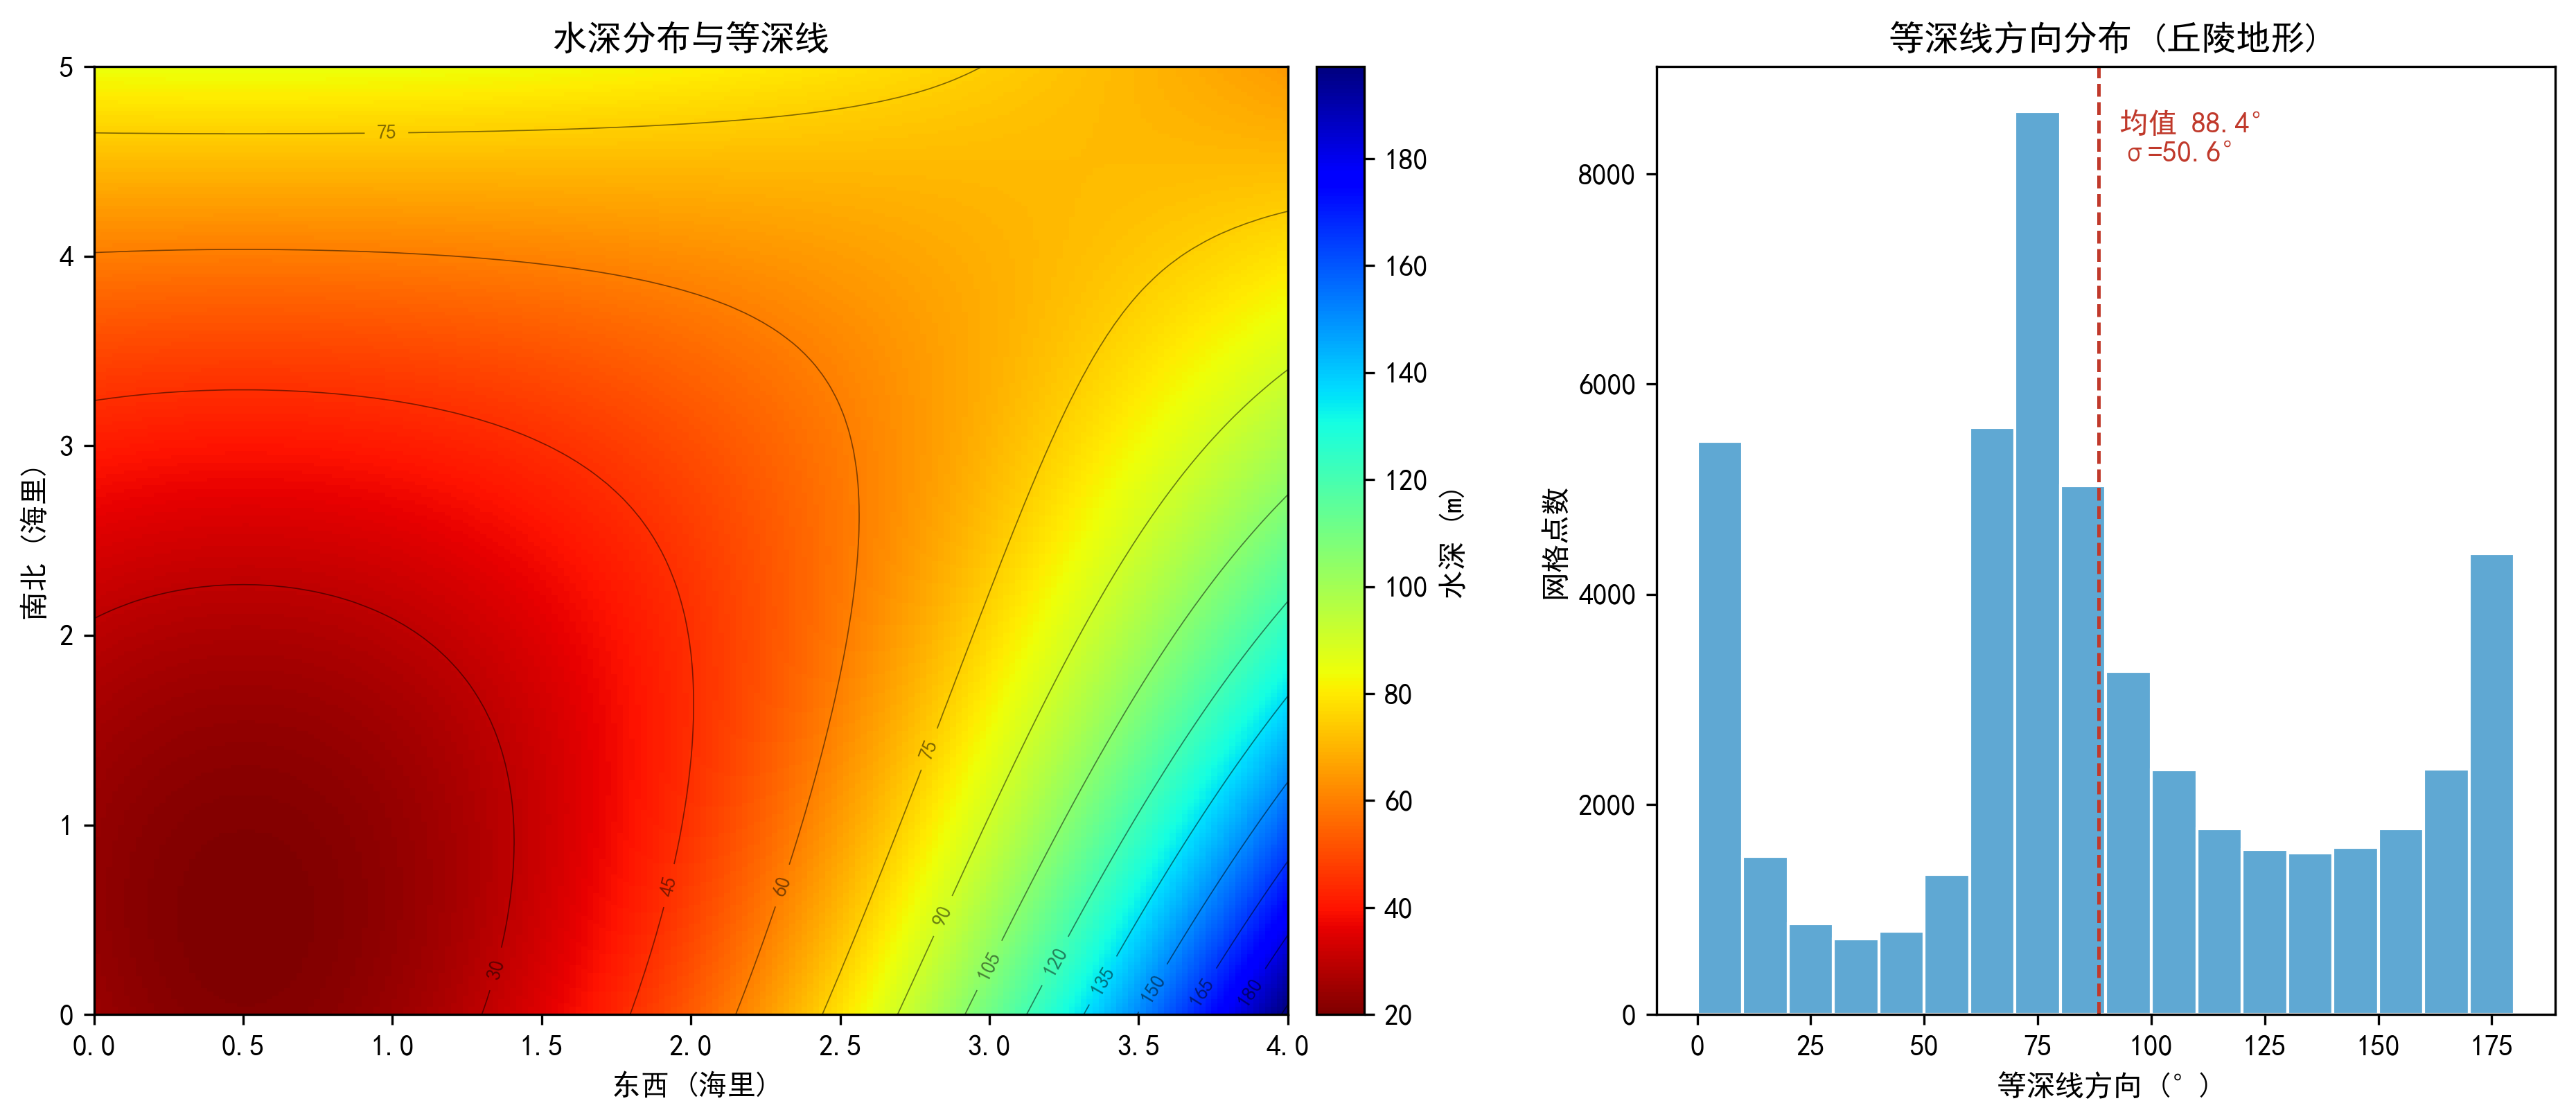
\includegraphics[width=0.95\textwidth]{../fig/fig_q4_terrain.png}
\caption{第四问海域地形特征（水深分布与等深线、等深线方向分布）}
\label{fig:q4-terrain}
\end{figure}


\subsubsection{模型构建}

\textbf{1. 方向相关的条带宽度场}

第三问的解析模型（式 \ref{eq:width}）要求坡度恒定；真实地形中坡度逐点变化，
需将模型推广为逐点、逐方向的宽度场。测线法线方向为 $(n_x,n_y)$ 时，
视坡角为地形梯度在该方向的投影 $\tan\alpha' = |g_x n_x + g_y n_y|$，
代入式 (\ref{eq:width}) 得方向相关的条带宽度场：
\begin{equation}
    \tan\alpha' = |g_x n_x + g_y n_y|, \qquad
    W_\theta(x,y) = H(x,y)\left[\frac{1}{\tan30^\circ+\tan\alpha'}+\frac{1}{\tan30^\circ-\tan\alpha'}\right]
\end{equation}
$W_\theta$ 的意义：测线方向为 $\theta$（法线方向 $n_\theta$）时，
位置 $(x,y)$ 处的条带宽度。由于平均坡度仅 0.83°（$\tan\alpha'\le0.015$），
方向对视坡角、进而对宽度的影响小于 5\%——
方向优化的收益主要来自覆盖几何（线族穿越深度带的平滑性）而非宽度本身，
但宽度场仍随方向变化，须在布设时逐方向计算。

\textbf{2. 平行线族布设模型}

对候选方向 $\theta$，其法线方向为 $n_\theta=(-\sin\theta,\cos\theta)$，
测线族用法线坐标 $c=n_\theta\cdot P$ 参数化。自 $c_{\min}$ 端起步，
首线覆盖该侧边界，随后按"间距 $=0.9\times$ 线上宽度分位数"沿法线推进，
直至覆盖 $c_{\max}$ 侧边界。
每条测线的宽度代表值取该测线所经网格点宽度场 $W_\theta$ 的分位数——
用分位数而非最小值，是避免个别浅脊点把整条间距锁死（见分位权衡）。
以漏测率 $\mathcal{M}(\theta)$ 度量方向 $\theta$ 的布设质量，
最优方向为 $\theta^*=\arg\min\mathcal{M}(\theta)$。

\textbf{3. 间距分位模型}

真实地形中漏测呈\textbf{碎片化}分布（以 90° 方向、0.5 分位间距的布设为例，
漏测网格形成 954 个连通块、且全部不大于 7 个网格）——
漏测由个别浅脊/深谷处的局部宽度不足造成，无法通过"块中心补线"
（补线成本高、收益极小）修复，只能通过收紧间距分位控制。
间距取线上宽度场的分位数 $\rho$（$\rho$ 越小间距越保守），
分位取值构成漏测率与总长的权衡，$\rho$ 的选择见结果分析。

\textbf{4. 指标定义}

三个题定指标的网格化计算口径：
\begin{enumerate}
    \item \textbf{测线总长度}：各测线在海域内的截线长度之和；
    \item \textbf{漏测率}：网格点被任一条带覆盖的判定为 $d(P,L_i)\le W_\theta(P)/2$
      （$d$ 为点到测线最近距离），漏测率 $=$ 未覆盖网格数 $/$ 总网格数；
    \item \textbf{超 20\% 重叠长度}：对测线上每个采样点，重叠率
      $\eta=1-d/W_{\min}$（$W_{\min}$ 为相邻两条中较浅者的宽度），
      将 $\eta>0.2$ 的测线弧长累计。
\end{enumerate}

\subsubsection{求解方法}

\textbf{步骤一：方向扫描。}对 $\theta\in[85^\circ,125^\circ]$ 每 $5^\circ$ 一次
（覆盖等深线均值 88.4° 及其两侧），按平行线族布设模型逐方向布设，
统计各方向的漏测率与总长，取漏测率最小的方向为最优方向。

\textbf{步骤二：分位权衡。}对最优方向，取 $\rho\in\{0.3,0.35,0.4,0.5\}$
分别布设，计算漏测率与总长，在"漏测率 $<1\%$"约束下选取总长
最短的分位（帕累托最优点）。

\textbf{步骤三：PWS 方法学检验。}作为方法学对比，实现文献中
"惩罚加权最短路径"（PWS）迭代法。PWS 框架以 8 邻域网格图为载体，
边权由三项叠加：
\begin{equation}
    w(e) = \ell(e)\left[1 + k\sin^2(\theta_e - \theta_{\text{iso}})\right] + C_{\text{cov}}
\end{equation}
其中 $\ell(e)$ 为边长，第二项为方向惩罚（偏离等深线方向的加权，
$k=3$，引导测线贴合等深线），$C_{\text{cov}}$ 为覆盖惩罚
（进入已覆盖条带区的碗形惩罚，随迭代累加）。
每次迭代以 Dijkstra\cite{bib:dijkstra} 求一条贯穿南北的最小权重路径作为新测线，
更新覆盖惩罚后重复，直至覆盖饱和。三个变体（贴合等深线、
平滑曲率约束、覆盖引导）与贪心方案的结果对比见结果分析。

\subsubsection{结果分析}

\textbf{1. 方向扫描结果}

方向扫描显示：$\theta=105^\circ\sim110^\circ$ 漏测率最低（约 2.8\%），
显著优于南北向 90°（5.1\%）。机理：对地形分区统计等深线方向，
西区（浅水）均值 103°、东区（深水）均值 79°，东西分区方向差达 24°——
单一方向无法同时贴合两区，全局折中的 105° 线族使各线穿越深度带的
平滑性最优、覆盖死角最少。\textbf{该结果说明真实地形的"最优测线方向"
不是简单沿用第三问的 90°}，而是地形结构（等深线方向分布）的函数。

\textbf{2. 分位权衡结果}

间距分位 $\rho$ 的权衡如表~4 所示：

\begin{table}[htbp]
\centering
\caption{间距分位权衡（$\theta=105^\circ$）}
\label{tab:q4-quantile}
\begin{tabular}{cccc}
\toprule[1.5pt]
分位 $\rho$ & 条数 & 总长（海里） & 漏测率 \\ \midrule[1pt]
0.5（宽松） & 77 & 248.3 & 2.77\% \\
0.4 & 80 & 264.2 & 1.04\% \\
\textbf{0.35（采用）} & \textbf{77} & \textbf{276.2} & \textbf{0.44\%} \\
0.3（保守） & 83 & 278.0 & 0.21\% \\
\bottomrule[1.5pt]
\end{tabular}
\end{table}

漏测率每降一个数量级需付出总长与重叠率的代价（三角权衡不可兼得）：
$\rho=0.5\to0.3$ 时漏测率 2.77\%$\to$0.21\%，代价是总长
248.3$\to$278.0 海里、超 20\% 重叠长度同步上升。
\textbf{$\rho=0.35$ 是"漏测率 $<1\%$"约束下总长最短的帕累托最优点}，
即漏测约束收紧时最经济的分位选择。

\textbf{3. 最终方案结果}

最终方案：测线方向 $105^\circ$，77 条测线，总长 276.24 海里，
漏测率 0.44\%，重叠率超过 20\% 部分的总长度 116.98 海里。
与同分位口径的 90° 方案相比，总长 290.00$\to$276.24 海里（$-4.7\%$）、
超 20\% 重叠 136.88$\to$116.98 海里（$-14.5\%$）、漏测率 0.85\%$\to$0.44\%，
三个指标全面改善，且漏测率满足 $<1\%$ 的工程要求。测线布局如图~\ref{fig:q4-layout} 所示。

\begin{figure}[htbp]
\centering
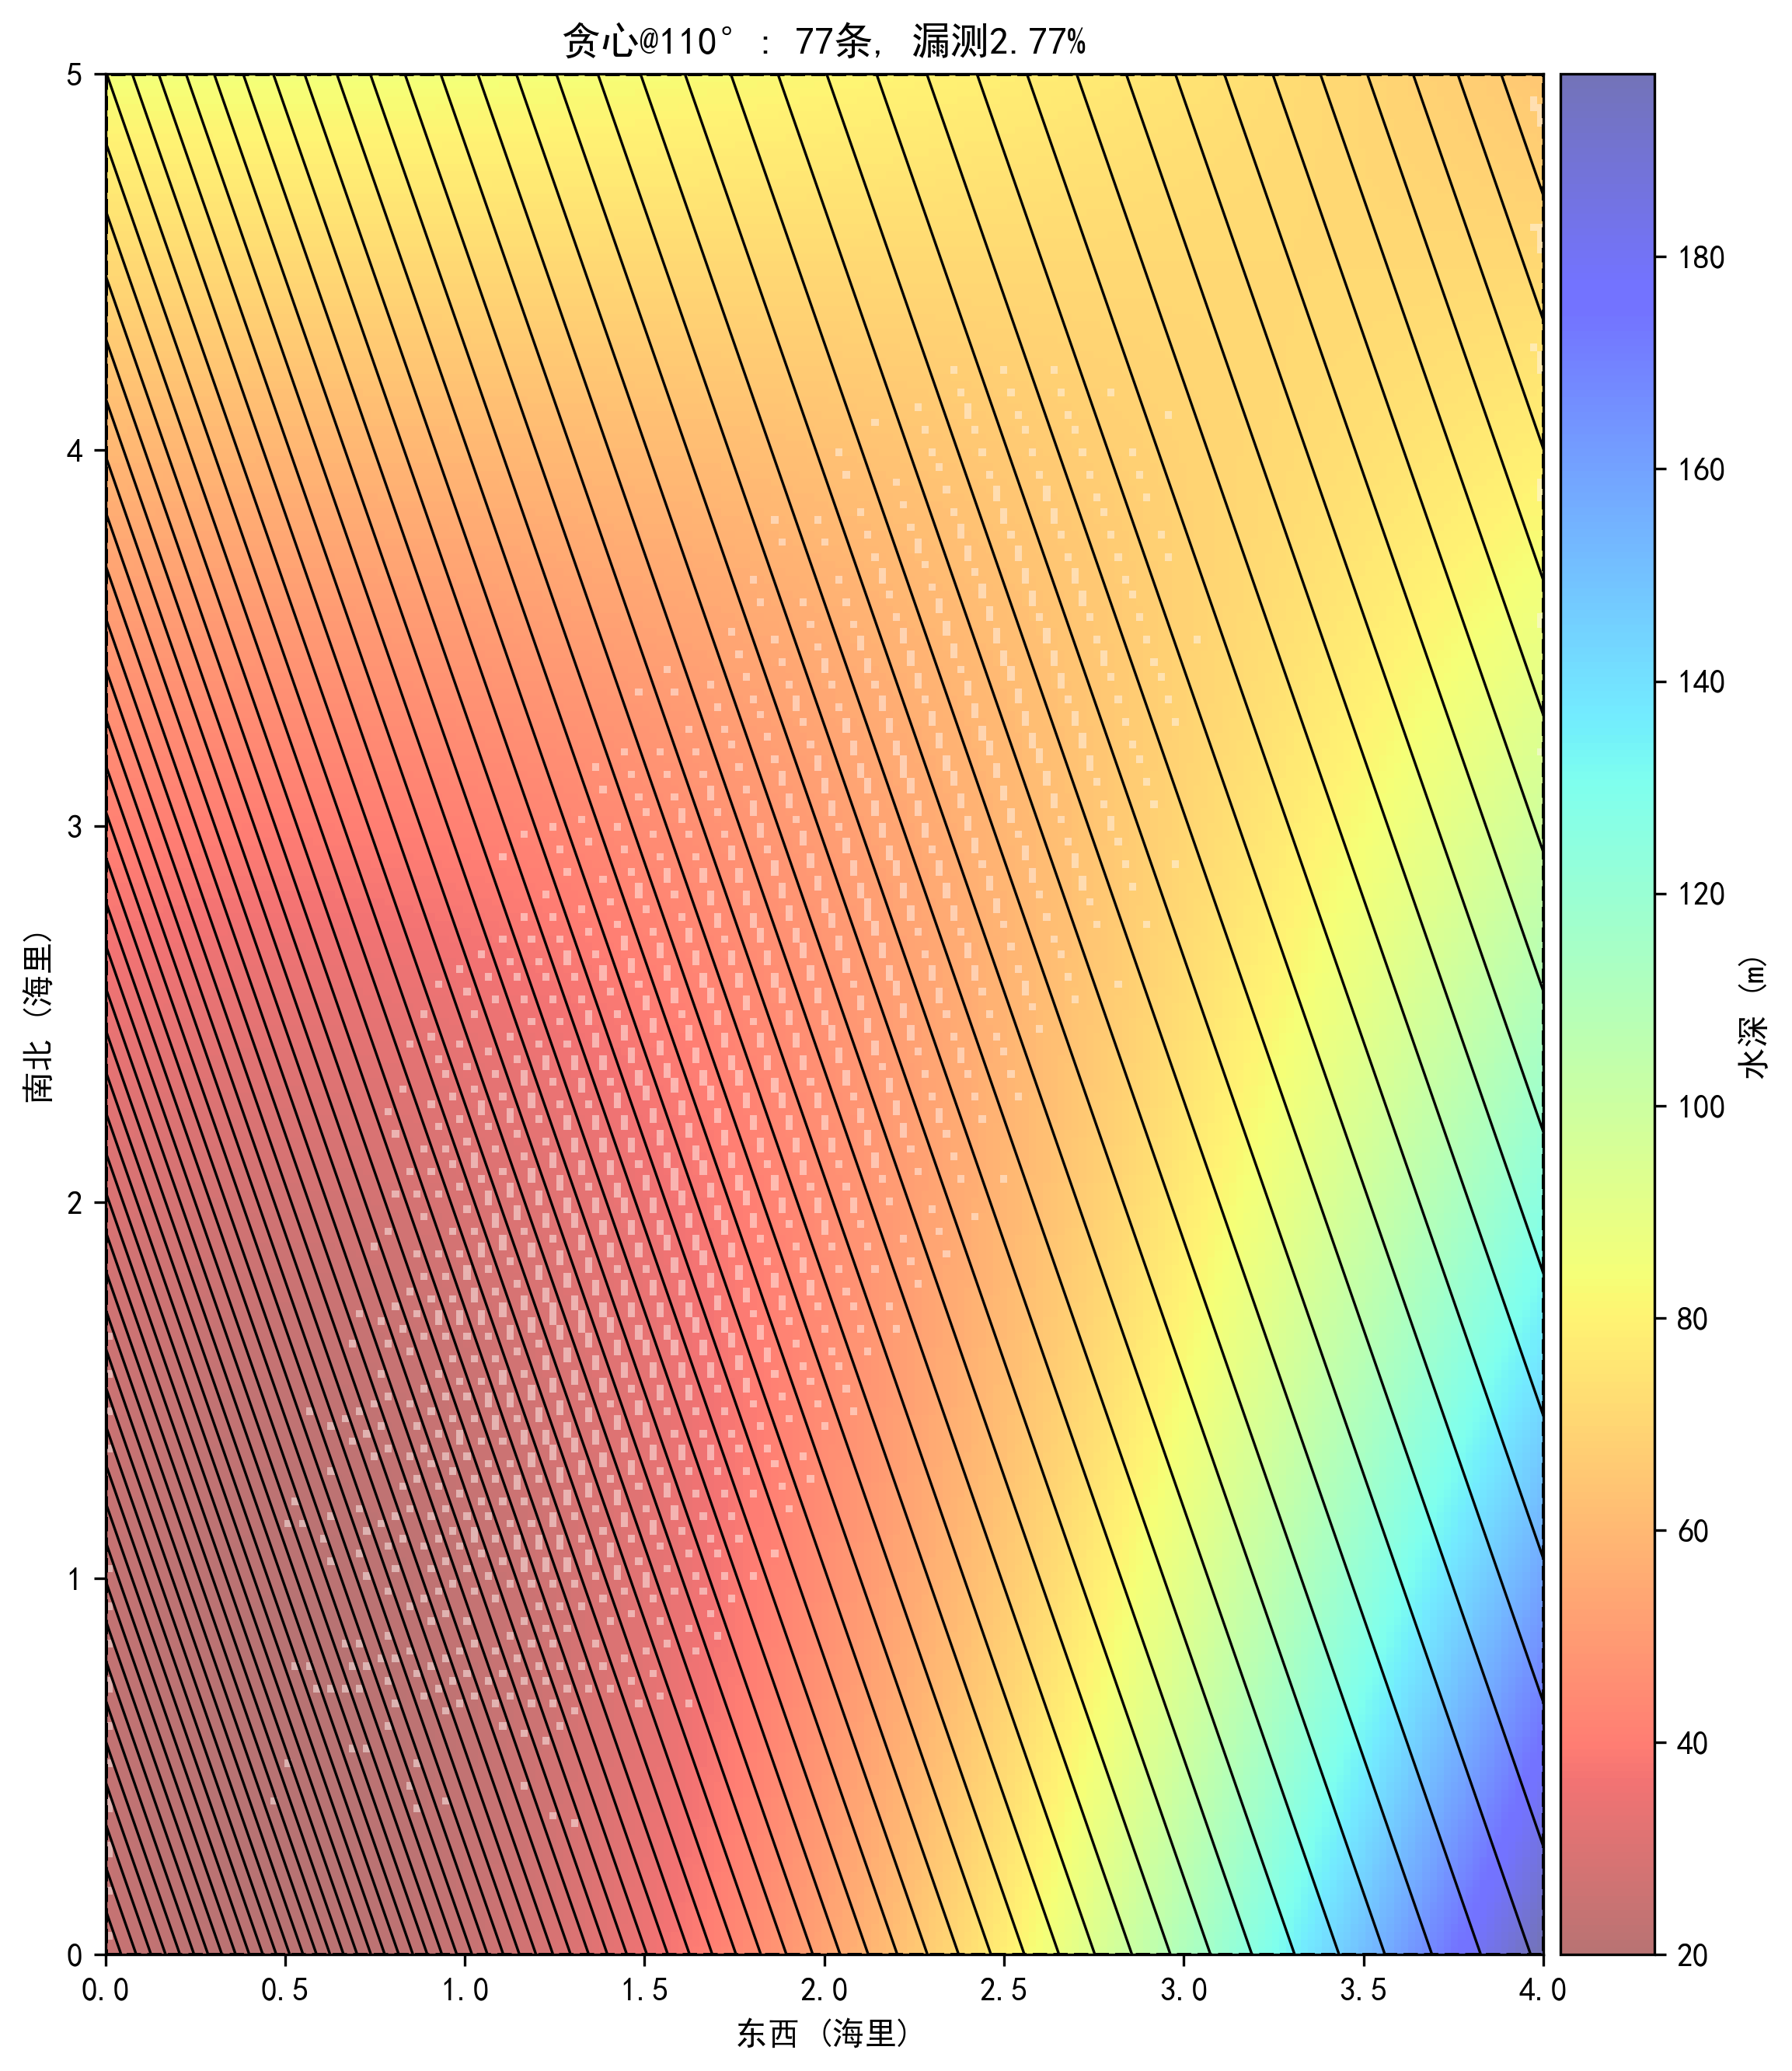
\includegraphics[width=0.85\textwidth]{../fig/fig_q4_layout.png}
\caption{第四问 $105^\circ$ 斜线族测线布局（黑：主线，红：漏测区）}
\label{fig:q4-layout}
\end{figure}


\textbf{4. 方法对比与机理分析}

四个方法（贪心主方案 + PWS 三变体）的指标对比如表~5 所示：

\begin{table}[htbp]
\centering
\caption{第四问各方法指标对比}
\label{tab:q4-methods}
\begin{tabular}{ccccc}
\toprule[1.5pt]
算法 & 条数 & 总长（海里） & 漏测率 & 超 20\% 重叠（海里） \\ \midrule[1pt]
\textbf{贪心@105°（主方案）} & \textbf{77} & \textbf{276.2} & \textbf{0.44\%} & \textbf{117.0} \\
PWS-贴合等深线 & 68 & 415.6 & 1.96\% & 355.9 \\
PWS-平滑（曲率约束） & 66 & 392.7 & 1.96\% & 327.1 \\
PWS-覆盖引导（目标修正） & 45 & 234.3 & 12.41\% & 111.0 \\
\bottomrule[1.5pt]
\end{tabular}
\end{table}

\begin{figure}[htbp]
\centering
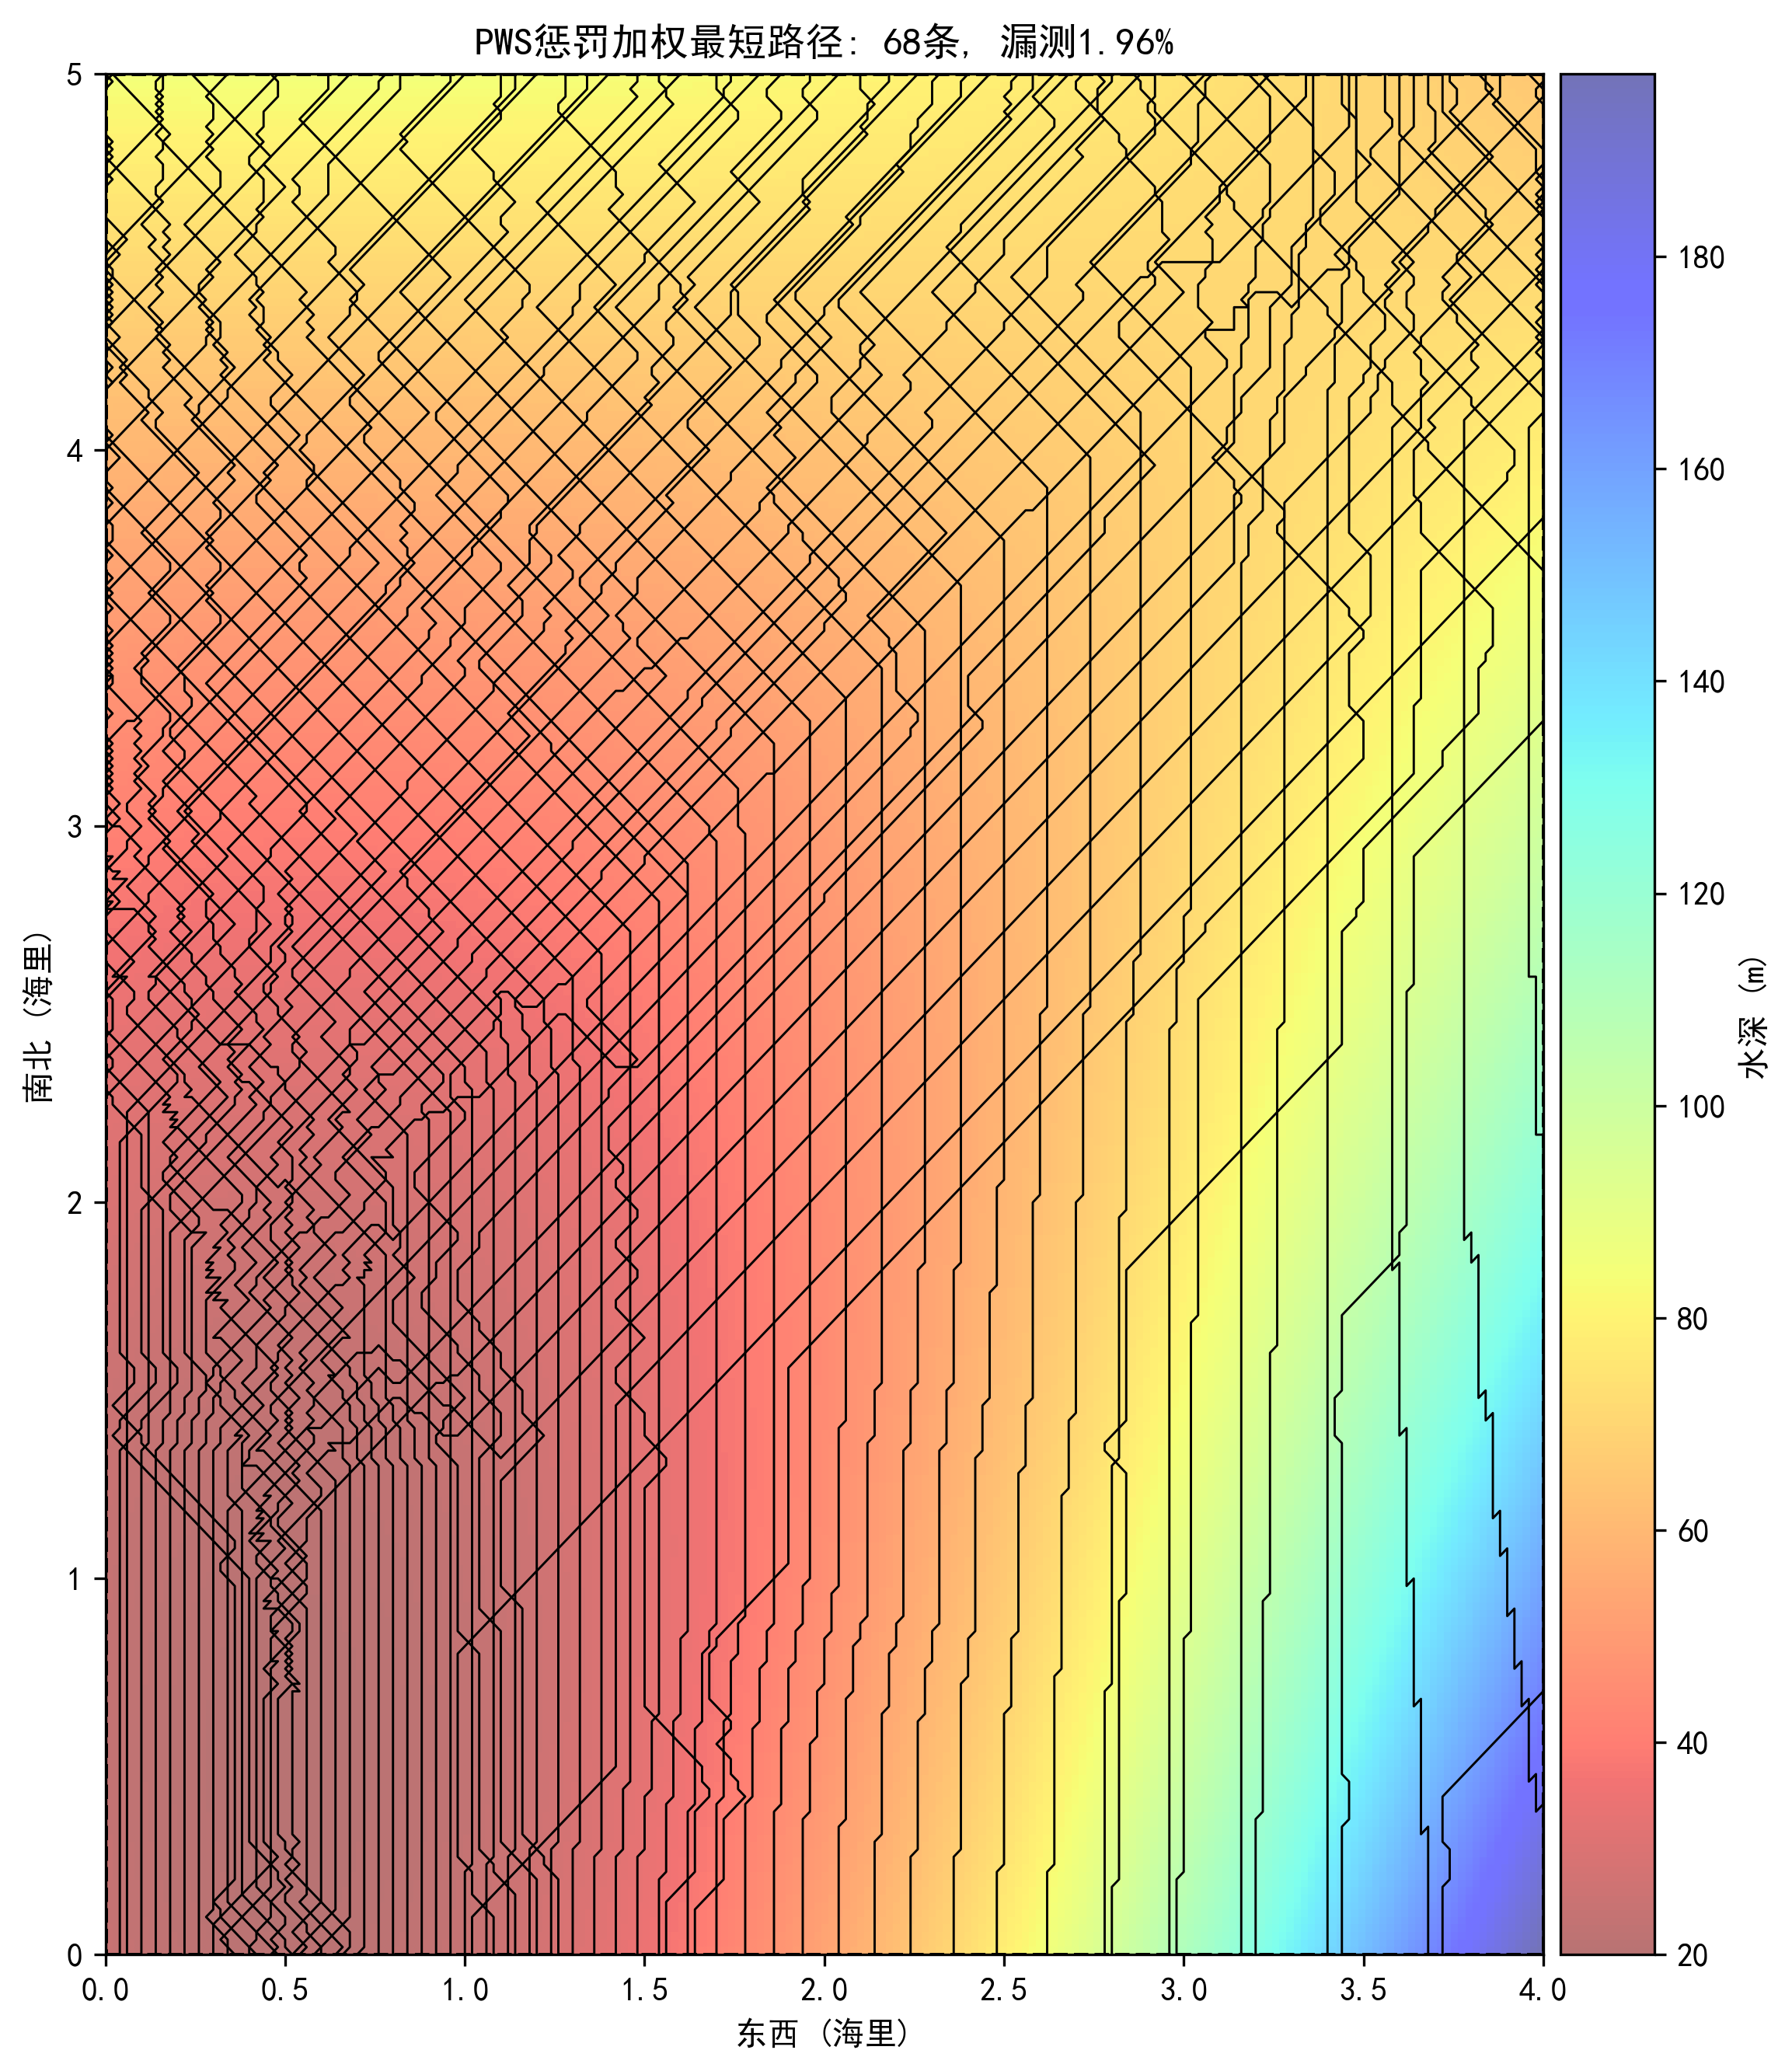
\includegraphics[width=0.85\textwidth]{../fig/fig_q4_pws.png}
\caption{PWS 曲线测线方案（测线蜿蜒贴合等深线）}
\label{fig:q4-pws}
\end{figure}

PWS 各变体的系统性劣势揭示了重要的机理结论：

（1）\textbf{贴合等深线版}——方向惩罚使测线贴合蜿蜒的等深线
（等深线方向标准差 50.6°），曲线测线随之大幅弯曲，相邻曲线间的
法向距离沿程剧烈变化：收拢段重叠率爆炸（超 20\% 重叠 355.9 海里，
为贪心方案的 3 倍）、张开段漏测，同时弯曲使单线更长，总长劣化 50\%；

（2）\textbf{平滑版}——对路径施加移动平均平滑（惩罚不增约束）
仅改善 5\%$\sim$8\%，证明弯曲是等深线固有的\textbf{长波}特征而非
网格离散锯齿，曲率约束无法根本修复；

（3）\textbf{覆盖引导版}——将目标修正为"最短路径 + 避重叠"
（去掉方向惩罚、禁止进入已覆盖区）后，测线近似直线且位置由
未覆盖走廊自适应确定，总长反超贪心（234.3 vs 276.2 海里）、
重叠率与贪心相当，但漏测率升至 12.4\%——单目标最优导致
三目标失衡。

上述对比得到核心机理结论：\textbf{贪心的优势来自显式间距递推
（$d=0.9W_{\min}$ 逐条锁定间距），而曲线测线族的间距是地形曲率的函数，
PWS 类方法的软惩罚无法在碎片化未覆盖区维持间距均匀}；
PWS-覆盖引导版的"总长反超"则说明 Dijkstra 框架的价值在于
全局最短路径搜索，与显式间距控制互补而非替代。PWS 曲线测线方案如图~\ref{fig:q4-pws} 所示。





\section{模型检验与灵敏度分析}

\subsection{问题三的重叠率灵敏度}

重叠率设计下界每放宽 5\%（间距系数 0.9$\to$0.85$\to$0.8），
测线条数 36$\to$37$\to$40，总长 72$\to$74$\to$80 海里。
工程上若考虑条带宽度 $\pm5\%$ 的测量误差，设计重叠率宜取 15\% 以留鲁棒余量，
对应 37 条测线、总长 74 海里。

\subsection{问题四的鲁棒性}

（1）方向敏感性：$\theta\in[100^\circ,115^\circ]$ 内总长变化小于 4\%，方案对方向不敏感；
（2）分位敏感性：$\rho\in[0.3,0.4]$ 内漏测率 0.21\%$\sim$1.04\%，
总长变化小于 3\%，方案稳健
（三指标的计算口径见问题四模型构建中"指标定义"部分）。

\section{模型评价与改进}

\subsection{模型优点}

\begin{enumerate}
    \item 问题一至三模型为解析式，几何意义明确、可解释性强，
          与数值模拟结果完全一致；
    \item 重叠率"瓶颈口径"贯穿四个问题，设计约束与指标定义全局自洽；
    \item 问题四采用"方向扫描 + 间距分位 + 多方法对比"的完整框架，
          覆盖几何优化、鲁棒性分析与方法学检验三个层次；
    \item 三算法验证（贪心/DP/GA）与 PWS 三变体对比，
          结论均有量化数据支撑。
\end{enumerate}

\subsection{模型改进}

\begin{enumerate}
    \item \textbf{引入重叠率逐点自适应间距}：第四问中重叠率沿测线变化，
      可将测线间距改进为随深度分段调整（分段常数间距），
      进一步压缩超 20\% 重叠长度；
    \item \textbf{曲线测线可行性研究}：PWS-覆盖引导版的总长优势提示，
      若对曲线测线增加"间距均匀性"硬约束（如路径平滑 + 法向等距重采样），
      曲线方案有望在保证覆盖的前提下优于直线方案；
    \item \textbf{航迹级联合优化}：将测线方向、间距与蛇形折返转弯段
      纳入统一的路径规划框架（TSP 变体），追求完整航迹（而非测线）最短；
    \item \textbf{误差传播分析}：考虑波束开角误差、测深误差与船位误差对
      覆盖宽度与重叠率的传播影响，以蒙特卡洛方法给出设计重叠率的
      置信区间推荐值。
\end{enumerate}

%参考文献
\begin{thebibliography}{9}%宽度9
    \bibitem{bib:lidong}
    李家彪. 多波束勘测原理技术与方法[M]. 北京: 海洋出版社, 1999.

    \bibitem{bib:zhao}
    赵建虎, 刘经南. 多波束测深及图像数据处理[M]. 武汉: 武汉大学出版社, 2008.

    \bibitem{bib:dijkstra}
    Dijkstra E W. A note on two problems in connexion with graphs[J].
    Numerische Mathematik, 1959, 1(1): 269--271.

    \bibitem{bib:gb}
    中华人民共和国国家标准. 海道测量规范: GB 12327--1998[S].
    北京: 中国标准出版社, 1998.
\end{thebibliography}

\newpage

%附录
\begin{appendices}

\section{问题一：覆盖宽度与重叠率计算（完整代码 solve\_q1.py）}

\begin{lstlisting}[language=python]

"""
2023B多波束测线 第一问计算
D0=70m, α=1.5°, 开角120°(边缘与竖直60°), 测线间距d=200m
W = D·[1/(tan30°+tanα) + 1/(tan30°-tanα)]
η = 1 - d/W_prev
用法: python solve_q1.py [--write]
"""
import argparse
from pathlib import Path

import numpy as np

ROOT = Path(__file__).resolve().parent.parent   # 单刷2023B/
RESULT = ROOT / 'result1.xlsx'

D0 = 70.0
ALPHA = np.deg2rad(1.5)
D_LINE = 200.0
X = np.array([-800, -600, -400, -200, 0, 200, 400, 600, 800])


def depth(x):
    return D0 - x * np.tan(ALPHA)          # x正方向为坡上(浅侧)


def width(D):
    t30 = np.tan(np.pi / 6)
    return D * (1 / (t30 + np.tan(ALPHA)) + 1 / (t30 - np.tan(ALPHA)))


def main(write=False):
    Ds = depth(X)
    Ws = width(Ds)
    print(f"{'位置/m':>7} {'水深/m':>9} {'W/m':>9} {'重叠率':>8}")
    for i, (x, d, w) in enumerate(zip(X, Ds, Ws)):
        eta = '——' if i == 0 else (
            f"{1 - D_LINE/Ws[i]:.2%}" if 1 - D_LINE/Ws[i] >= 0 else '无重叠')
        print(f"{x:>7} {d:>9.2f} {w:>9.2f} {eta:>8}")

    if write:
        from openpyxl import load_workbook
        wb = load_workbook(RESULT)
        ws = wb.active
        for i in range(len(X)):
            ws.cell(2, i + 2).value = round(Ds[i], 2)
            ws.cell(3, i + 2).value = round(Ws[i], 2)
            if i > 0:
                e = 1 - D_LINE / Ws[i]
                ws.cell(4, i + 2).value = '无重叠' if e < 0 else f'{e:.2%}'
        wb.save(RESULT)
        print(f'[OK] 写入 {RESULT}')


if __name__ == '__main__':
    p = argparse.ArgumentParser()
    p.add_argument('--write', action='store_true')
    main(write=p.parse_args().write)

\end{lstlisting}

\section{问题二：覆盖宽度 W(L,β) 计算（完整代码 solve\_q2.py）}

\begin{lstlisting}[language=python]

"""
2023B多波束测线 第二问计算
β: 测线方向与坡面法向水平投影的夹角; L: 测线上距中心点距离(海里)
H(L,β) = H0 - L·tanα·cosβ
tanα' = tanα·|sinβ|
W = H·[1/(tan30°+tanα') + 1/(tan30°-tanα')]
用法: python solve_q2.py [--write]
"""
import argparse
from pathlib import Path

import numpy as np

ROOT = Path(__file__).resolve().parent.parent
RESULT = ROOT / 'result2.xlsx'

H0 = 120.0          # 中心点水深 (m)
ALPHA = np.deg2rad(1.5)
NM = 1852.0         # 1海里 = 1852m
BETA = np.array([0, 45, 90, 135, 180, 225, 270, 315])
L_NM = np.array([0, 0.3, 0.6, 0.9, 1.2, 1.5, 1.8, 2.1])

t30 = np.tan(np.pi / 6)
ta = np.tan(ALPHA)


def width(H, ta_p):
    return H * (1 / (t30 + ta_p) + 1 / (t30 - ta_p))


def main(write=False):
    W = np.zeros((len(BETA), len(L_NM)))
    for i, b in enumerate(BETA):
        cb, sb = np.cos(np.deg2rad(b)), np.sin(np.deg2rad(b))
        ta_p = ta * abs(sb)                     # 视坡角
        for j, lnm in enumerate(L_NM):
            H = H0 - lnm * NM * ta * cb         # 沿测线水深
            W[i, j] = width(H, ta_p)

    print(f"{'β\\L(海里)':>9}" + "".join(f"{l:>9.1f}" for l in L_NM))
    for i, b in enumerate(BETA):
        print(f"{b:>9.0f}" + "".join(f"{W[i, j]:>9.2f}" for j in range(len(L_NM))))

    if write:
        from openpyxl import load_workbook
        wb = load_workbook(RESULT)
        ws = wb.active
        for i in range(len(BETA)):
            for j in range(len(L_NM)):
                ws.cell(3 + i, 3 + j).value = round(W[i, j], 2)
        wb.save(RESULT)
        print(f'[OK] 写入 {RESULT}')


if __name__ == '__main__':
    p = argparse.ArgumentParser()
    p.add_argument('--write', action='store_true')
    main(write=p.parse_args().write)

\end{lstlisting}

\section{问题三：测线布设与航迹分析（完整代码 solve\_q3.py）}

\begin{lstlisting}[language=python]

"""
2023B多波束测线 第三问最终版
海域: 南北2海里×东西4海里, 西深东浅, 中心水深110m, α=1.5°, 开角120°
目标: 总测线长度最短 + 全覆盖 + 重叠率10%~20%

建模链:
  ① 方向优化: 扫描β(测线与坡上方向夹角), 证明β=90°(沿等深线)最短
  ② 起点验证: 深水端/浅水端起步同口径对比, 条数相同, 取深水端
  ③ 间距推导: 重叠率≥10%反解 d=0.9·W_瓶颈(相邻两条中较浅者)
  ④ 最终方案: 36条南北向测线, 总长72海里, 重叠率恰10%

用法: python solve_q3.py
"""
import numpy as np

H0 = 110.0
ALPHA = np.deg2rad(1.5)
NM = 1852.0
W_NS, W_EW = 2 * NM, 4 * NM
XW, XE = -W_EW / 2, W_EW / 2
t30 = np.tan(np.pi / 6)
ta = np.tan(ALPHA)
K = 1 / (t30 + ta) + 1 / (t30 - ta)


def depth(x):
    return H0 - x * ta                      # x向东为正, 西深东浅


def width(x):
    return K * depth(x)


# ============ ① 方向优化 (扫描β, 相对总长) ============
def simulate_beta(beta_deg):
    """给定β模拟布设(深水端起步), 返回总长海里。
    间距用当前测线浅端W——仅用于方向相对比较。"""
    beta = np.deg2rad(beta_deg)
    t = np.array([np.cos(beta), np.sin(beta)])
    n = np.array([-np.sin(beta), np.cos(beta)])
    corners = np.array([[W_EW/2, W_NS/2], [W_EW/2, -W_NS/2],
                        [-W_EW/2, -W_NS/2], [-W_EW/2, W_NS/2]])
    cn = corners @ n
    cmin, cmax = cn.min(), cn.max()

    def line(c):
        """测线n·P=c与矩形交线段: (长度, 浅端水深)"""
        ss = []
        for p1, p2 in [((W_EW/2, -W_NS/2), (W_EW/2, W_NS/2)),
                       ((-W_EW/2, -W_NS/2), (-W_EW/2, W_NS/2)),
                       ((-W_EW/2, W_NS/2), (W_EW/2, W_NS/2)),
                       ((-W_EW/2, -W_NS/2), (W_EW/2, -W_NS/2))]:
            p1, p2 = np.array(p1, float), np.array(p2, float)
            d = p2 - p1
            M = np.array([[t[0], -d[0]], [t[1], -d[1]]])
            bv = np.array([p1[0] - c * n[0], p1[1] - c * n[1]])
            try:
                s, u = np.linalg.solve(M, bv)
            except np.linalg.LinAlgError:
                continue
            if -1e-6 <= u <= 1 + 1e-6:
                ss.append(s)
        if len(ss) < 2:
            return 0.0, 1e9
        s_lo, s_hi = min(ss), max(ss)
        xm = max(c*n[0] + s_lo*t[0], c*n[0] + s_hi*t[0])
        return (s_hi - s_lo), max(H0 - xm * ta, 1.0)

    c_west = [-W_EW/2 * n[0] + W_NS/2 * n[1],
              -W_EW/2 * n[0] - W_NS/2 * n[1]]
    start_is_min = (min(c_west) - cmin) < (cmax - max(c_west))
    c_start, c_end = (cmin, cmax) if start_is_min else (cmax, cmin)
    sgn = 1 if c_end > c_start else -1

    c1 = c_start
    for _ in range(30):                     # 第一条: 覆盖深水端角点
        _, Hm = line(c1)
        c1_new = c_start + sgn * K * Hm / 2
        if abs(c1_new - c1) < 1.0:
            break
        c1 = c1_new

    cs, guard = [c1], 0
    while sgn * (cs[-1] - c_end) < -1e-3:
        guard += 1
        if guard > 3000:
            break
        _, Hm = line(cs[-1])
        cs.append(cs[-1] + sgn * max(0.9 * K * Hm, 0.1))
    return sum(line(c)[0] for c in cs) / NM


def direction_scan():
    print("=" * 50)
    print("① 方向优化: 相对总长 vs β (β=90°为基准1.00)")
    print("=" * 50)
    l90 = simulate_beta(90)
    for b in range(0, 181, 15):
        lb = simulate_beta(b)
        mark = '  ← 最短' if b == 90 else ''
        print(f"  β={b:>3}°: 相对{lb/l90:>6.2f}{mark}")
    print("  → 结论: β=90°(沿等深线南北向) 总长最短")


# ============ ② 起点验证 (同口径) ============
def layout_west():
    """深水(西)起步: 第一条覆盖西边界, 间距=0.9·W(下一条, 较浅)"""
    x1 = (XW + K * H0 / 2) / (1 + K * ta / 2)
    xs = [x1]
    while True:
        xn = (xs[-1] + 0.9 * K * H0) / (1 + 0.9 * K * ta)
        xs.append(xn)
        if xn + width(xn) / 2 >= XE:
            break
    return xs


def layout_east():
    """浅水(东)起步: 第一条覆盖东边界, 间距=0.9·W(当前线, 较浅)"""
    x1 = (XE - K * H0 / 2) / (1 - K * ta / 2)
    xs = [x1]
    while True:
        xn = xs[-1] - 0.9 * width(xs[-1])
        xs.append(xn)
        if xn - width(xn) / 2 <= XW:
            break
    return xs


def start_check():
    print()
    print("=" * 50)
    print("② 起点验证: 深水端 vs 浅水端 (同口径: d=0.9·min(W相邻))")
    print("=" * 50)
    for name, xs in [("深水(西)端", layout_west()), ("浅水(东)端", layout_east())]:
        print(f"  {name}起步: {len(xs)}条, {len(xs)*W_NS/NM:.0f}海里")
    print("  → 结论: 条数相同, 取深水端为布设起点")


# ============ ③④ 最终方案 ============
def final_layout():
    print()
    print("=" * 50)
    print("③④ 最终布设 (深水端起步, d=0.9·W_瓶颈)")
    print("=" * 50)
    xs = np.array(layout_west())
    d = np.diff(xs)
    eta = [1 - d[i] / width(xs[i + 1]) for i in range(len(d))]
    print(f"  测线方向: 南北向(沿等深线), {len(xs)}条, "
          f"总长{len(xs)*W_NS/NM:.0f}海里")
    print(f"  {'#':>3} {'x/m':>8} {'水深/m':>8} {'W/m':>8} {'间距/m':>8} "
          f"{'重叠率':>8}")
    print("  " + "-" * 50)
    for i in range(len(xs)):
        if i == 0:
            print(f"  {i+1:>3} {xs[i]:>8.1f} {depth(xs[i]):>8.1f} "
                  f"{width(xs[i]):>8.1f} {'--':>8} {'--':>8}")
        else:
            print(f"  {i+1:>3} {xs[i]:>8.1f} {depth(xs[i]):>8.1f} "
                  f"{width(xs[i]):>8.1f} {d[i-1]:>8.1f} {eta[i-1]*100:>7.2f}%")

    cw = xs[0] - width(xs[0]) / 2
    ce = xs[-1] + width(xs[-1]) / 2
    print(f"  验证: 西边界{cw:.1f}m(需≤{XW:.1f}), "
          f"东边界{ce:.1f}m(需≥{XE:.1f}), "
          f"重叠率{min(eta)*100:.1f}%~{max(eta)*100:.1f}% 通过")


# ============ ⑤ 航迹完整性: 蛇形折返转弯段 ============
def track_stat():
    print()
    print("=" * 50)
    print("⑤ 航迹完整性: 蛇形折返转弯航程 (测线外真实航行距离)")
    print("=" * 50)
    xs = np.array(layout_west())
    d = np.diff(xs)
    r_ideal = d / 2                      # 理想: 最小半径=间距/2
    r_real = np.maximum(r_ideal, 200.0)  # 保守: 船最小转弯半径200m
    L_line = len(xs) * W_NS
    t_ideal = np.pi * r_ideal.sum()
    t_real = np.pi * r_real.sum()
    # 对比: 梳形(每条从同端出发, L形连接段=东西间距+南北全宽)
    t_comb = len(d) * W_NS + d.sum()
    print(f"  测线长度: {L_line/NM:.0f} 海里")
    print(f"  蛇形转弯(理想r=d/2): {t_ideal/NM:.2f} 海里, "
          f"完整航迹 {(L_line+t_ideal)/NM:.1f} 海里")
    print(f"  蛇形转弯(保守R≥200m): {t_real/NM:.2f} 海里, "
          f"完整航迹 {(L_line+t_real)/NM:.1f} 海里")
    print(f"  对比-梳形(L形连接段): 完整航迹 {L_line/NM + t_comb/NM:.1f} 海里")
    print("  → 蛇形折返为最短连接方案(转弯占比7.7%, 梳形则近翻倍)")


if __name__ == '__main__':
    direction_scan()
    start_check()
    final_layout()
    track_stat()

\end{lstlisting}

\section{问题四：真实地形测线布设与多算法对比（完整代码 solve\_q4.py）}

\begin{lstlisting}[language=python]

"""
2023B第四问 真实地形测线布设 (附件.xlsx, 南北5海里×东西4海里)
算法:
  ① 方向扫描: θ∈[0,180) 平行线族贪心布设, 漏测率最小方向为最优
     (条带宽度用沿测线法线的视坡角, 方向相关)
  ② 贪心布设: 间距=0.9·线上W中位数, 逐条推进
  ③ 漏测修复: 漏测连通块中心沿主线方向补线
指标: 测线总长/漏测率/超20%重叠长度
用法: python solve_q4.py
"""
from pathlib import Path

import numpy as np
import pandas as pd
from scipy.spatial.distance import cdist

ROOT = Path(__file__).resolve().parent.parent
NM = 1852.0
t30 = np.tan(np.pi / 6)

# ===== 读取与地形场 =====
df = pd.read_excel(ROOT / '附件.xlsx', header=None)
H = df.iloc[2:, 2:].astype(float).values   # (251, 201) 行:南→北 列:西→东
NY, NX = H.shape
DX = 0.02 * NM
gy, gx = np.gradient(H, DX, DX)
GN = np.hypot(gx, gy)

n = NY * NX
Wr = (H * (1 / (t30 + GN) + 1 / (t30 - GN))).ravel()   # 沿梯度方向宽度(参考)
grid_y, grid_x = np.meshgrid(np.arange(NY) * DX, np.arange(NX) * DX,
                             indexing='ij')
GRID = np.stack([grid_x.ravel(), grid_y.ravel()], axis=1)   # (n, 2)

W_EW, W_NS = 4 * NM, 5 * NM
CORNERS = np.array([[0, 0], [W_EW, 0], [W_EW, W_NS], [0, W_NS]])
EDGES = [(0, 1), (1, 2), (2, 3), (3, 0)]


def w_field(nx, ny):
    """测线法线(nx,ny)方向的条带宽度场(视坡角=梯度沿法线投影)"""
    ta = np.abs(gx * nx + gy * ny)
    ta = np.minimum(ta, t30 * 0.99)
    return H * (1 / (t30 + ta) + 1 / (t30 - ta))


def solve_lines(theta_deg, quantile=0.35):
    """θ方向平行线族贪心布设: 间距=0.9·线上W分位数, 返回(lines, cov)"""
    th = np.deg2rad(theta_deg)
    t = np.array([np.cos(th), np.sin(th)])
    nv = np.array([-np.sin(th), np.cos(th)])
    Wth = w_field(nv[0], nv[1]).ravel()
    cn = CORNERS @ nv
    cmin, cmax = cn.min(), cn.max()

    def line(c):
        """法线nv·P=c 与海域的截线段(采样点)"""
        ss = []
        for a, b in EDGES:
            p1, p2 = CORNERS[a], CORNERS[b]
            denom = nv @ (p2 - p1)
            if abs(denom) < 1e-9:
                continue
            s = (c - nv @ p1) / denom
            if -1e-6 <= s <= 1 + 1e-6:
                ss.append(p1 + s * (p2 - p1))
        if len(ss) < 2:
            return None
        p, r = ss[0], ss[1]
        L = np.linalg.norm(r - p)
        k = max(2, int(L / DX))
        return p + np.linspace(0, 1, k)[:, None] * (r - p)

    lines, cov = [], np.zeros(n, bool)
    c = cmin
    while c < cmax - 1e-6:
        l = line(c)
        if l is None:
            break
        d = cdist(GRID, l).min(axis=1)
        cov |= (d <= Wth / 2)
        lines.append(l)
        idx = np.round(l[:, 1] / DX).astype(int) * NX + \
            np.round(l[:, 0] / DX).astype(int)
        c += 0.9 * np.percentile(Wth[idx], quantile * 100)
    return lines, cov


def repair_miss(lines, cov, theta_deg):
    """漏测连通块补线: 块中心沿主线方向θ补线"""
    from scipy import ndimage
    th = np.deg2rad(theta_deg)
    t = np.array([np.cos(th), np.sin(th)])
    for _ in range(6):
        cov2 = cov.reshape(NY, NX)
        lab, cnt = ndimage.label(~cov2, structure=np.ones((3, 3)))
        if cnt == 0:
            break
        m = 0
        for k in range(1, cnt + 1):
            ys, xs = np.where(lab == k)
            if len(ys) < 60:             # 微小块忽略
                continue
            pc = np.array([np.median(xs) * DX, np.median(ys) * DX])
            # 过pc沿θ的线与海域的交点
            ss = []
            for a, b in EDGES:
                p1, p2 = CORNERS[a], CORNERS[b]
                denom = t[0] * (p2[1] - p1[1]) - t[1] * (p2[0] - p1[0])
                if abs(denom) < 1e-9:
                    continue
                s = (t[0] * (p1[1] - pc[1]) - t[1] * (p1[0] - pc[0])) / denom
                if -1e-6 <= s <= 1 + 1e-6:
                    ss.append(p1 + s * (p2 - p1))
            if len(ss) < 2:
                continue
            p, r = ss[0], ss[1]
            L = np.linalg.norm(r - p)
            kk = max(2, int(L / DX))
            line = p + np.linspace(0, 1, kk)[:, None] * (r - p)
            lines.append(line)
            d = cdist(GRID, line).min(axis=1)
            cov |= (d <= Wr / 2)
            m += 1
        if m == 0:
            break
    return lines, cov


def metrics(lines, cov, theta_deg):
    """指标: 总长/漏测率/超20%重叠长度(逐点口径)"""
    th = np.deg2rad(theta_deg)
    nv = np.array([-np.sin(th), np.cos(th)])
    Wth = w_field(nv[0], nv[1]).ravel()

    def idx(pts):
        return np.round(pts[:, 1] / DX).astype(int) * NX + \
            np.round(pts[:, 0] / DX).astype(int)

    L = sum(np.linalg.norm(np.diff(l, axis=0), axis=1).sum() for l in lines)
    miss = 1 - cov.mean()
    over = 0.0
    for l in lines:
        O = np.concatenate([m for m in lines if m is not l], axis=0)
        dd = cdist(l, O)
        d = dd.min(axis=1)
        w_adj = Wth[idx(O[dd.argmin(axis=1)])]
        w_self = Wth[idx(l)]
        eta = 1 - d / np.minimum(w_self, w_adj)
        frac = (eta > 0.2).mean()
        over += frac * np.linalg.norm(np.diff(l, axis=0), axis=1).sum()
    return L / NM, miss, over / NM, len(lines)


def scan_direction():
    """方向扫描(漏测率最小者最优)"""
    best = (1e9, None)
    for th in range(85, 126, 5):
        _, cov = solve_lines(th)
        if 1 - cov.mean() < best[0]:
            best = (1 - cov.mean(), th)
    return best[1]


# ===== 对比算法: 惩罚加权最短路径(PWS)迭代Dijkstra =====
# 8邻域图, 边权=方向惩罚(贴合等深线)+覆盖惩罚(碗形), 迭代至覆盖饱和
from scipy.sparse import csr_matrix
from scipy.sparse.csgraph import dijkstra as sp_dijkstra

THETA_ISO = (np.arctan2(gy, gx) + np.pi / 2) % np.pi   # 等深线方向
K_DIR, P_COV = 3.0, 6000.0
rows, cols, wdir = [], [], []
for i in range(NY):
    for j in range(NX):
        u = i * NX + j
        for di, dj in ((0, 1), (1, 0), (1, 1), (1, -1)):
            ii, jj = i + di, j + dj
            if 0 <= ii < NY and 0 <= jj < NX:
                v = ii * NX + jj
                ell = np.hypot(di * DX, dj * DX)
                te = np.arctan2(di, dj)
                da = np.abs((te - THETA_ISO[(i + ii) // 2, (j + jj) // 2])
                            % np.pi)
                da = min(da, np.pi - da)
                w = ell * (1 + K_DIR * np.sin(da) ** 2)
                rows += [u, v]
                cols += [v, u]
                wdir += [w, w]
src, dst = n, n + 1
for j in range(NX):
    rows += [src, j, dst, (NY - 1) * NX + j]
    cols += [j, src, (NY - 1) * NX + j, dst]
    wdir += [0.0, 0.0, 0.0, 0.0]
rows, cols, wdir = np.array(rows), np.array(cols), np.array(wdir, float)

# 纯长度边权图(覆盖引导版PWS用, 无方向惩罚)
rows_l, cols_l, wlen = [], [], []
for i in range(NY):
    for j in range(NX):
        u = i * NX + j
        for di, dj in ((0, 1), (1, 0), (1, 1), (1, -1)):
            ii, jj = i + di, j + dj
            if 0 <= ii < NY and 0 <= jj < NX:
                ell = np.hypot(di * DX, dj * DX)
                rows_l += [u, ii * NX + jj]
                cols_l += [ii * NX + jj, u]
                wlen += [ell, ell]
for j in range(NX):
    rows_l += [src, j, dst, (NY - 1) * NX + j]
    cols_l += [j, src, (NY - 1) * NX + j, dst]
    wlen += [0.0, 0.0, 0.0, 0.0]
rows_l, cols_l, wlen = np.array(rows_l), np.array(cols_l), np.array(wlen, float)


def repair_dijkstra(lines, cov):
    """漏测块内Dijkstra补线: 禁入已覆盖区, 方向惩罚贴合局部地形
    对每个漏测连通块, 从块对应南边界区间到北边界区间找最短路径"""
    from scipy import ndimage
    for _ in range(6):
        cov2 = cov.reshape(NY, NX)
        lab, cnt = ndimage.label(~cov2, structure=np.ones((3, 3)))
        if cnt == 0:
            break
        m = 0
        for k in range(1, cnt + 1):
            ys, xs = np.where(lab == k)
            if len(ys) < 60:             # 微小块忽略
                continue
            jmin, jmax = int(xs.min()), int(xs.max())
            C = np.zeros(n + 2)
            C[:n] = 1e9 * cov.ravel()    # 已覆盖区禁入
            rows2 = list(rows) + [src] * (jmax - jmin + 1) \
                + [dst] * (jmax - jmin + 1)
            cols2 = list(cols) + list(range(jmin, jmax + 1)) \
                + [(NY - 1) * NX + j for j in range(jmin, jmax + 1)]
            w2 = np.concatenate([wdir, np.zeros(2 * (jmax - jmin + 1))])
            w2 = w2 + C[cols2]
            M = csr_matrix((w2, (rows2, cols2)), shape=(n + 2, n + 2))
            _, pred = sp_dijkstra(M, directed=False, indices=src,
                                  return_predecessors=True)
            path, u = [], dst
            while u != src and u != -1:
                path.append(u)
                u = pred[u]
            path = [v for v in path[::-1] if v < n]
            if not path:
                continue
            line = np.stack([GRID[v] for v in path])
            lines.append(line)
            d = cdist(GRID, line).min(axis=1)
            cov |= (d <= Wr / 2)
            m += 1
        if m == 0:
            break
    return lines, cov


def idx_fn(pts):
    """坐标→网格索引"""
    return np.round(pts[:, 1] / DX).astype(int) * NX + \
        np.round(pts[:, 0] / DX).astype(int)


def smooth_line(pts, C):
    """移动平均平滑: 抹平8邻域锯齿, 平滑点进入更深重叠区则回退"""
    pts = pts.copy()
    m = len(pts)
    for _ in range(3):
        new = pts.copy()
        for k in range(1, m - 1):
            cand = pts[max(0, k - 2):k + 3].mean(axis=0)
            ic = idx_fn(cand[None, :])[0]
            ik = idx_fn(pts[k:k + 1])[0]
            if C[ic] <= C[ik] + 1e-9:        # 惩罚不增: 不深入重叠区
                new[k] = cand
        pts = new
    return pts


def solve_pws_smooth(cov_target=0.98, max_iter=90):
    """PWS-平滑: 迭代Dijkstra + 移动平均平滑(曲率约束), 线更直间距更匀"""
    C = np.zeros(n + 2)
    cov = np.zeros(n, bool)
    lines = []
    for _ in range(max_iter):
        w = wdir + C[cols]
        M = csr_matrix((w, (rows, cols)), shape=(n + 2, n + 2))
        _, pred = sp_dijkstra(M, directed=False, indices=src,
                              return_predecessors=True)
        path, u = [], dst
        while u != src and u != -1:
            path.append(u)
            u = pred[u]
        path = [v for v in path[::-1] if v < n]
        pts = np.stack([GRID[v] for v in path])
        pts = smooth_line(pts, C)              # 平滑: 减少蛇形
        d = cdist(GRID, pts).min(axis=1)
        cov |= (d <= Wr / 2)
        lines.append(pts)
        C[:n] += P_COV * np.clip(0.9 * Wr - d, 0, None) / Wr
        if cov.mean() >= cov_target:
            break
    return lines, cov


def solve_pws(cov_target=0.98, max_iter=90):
    """PWS: 迭代Dijkstra, 覆盖碗形惩罚(间距落在0.9W)"""
    C = np.zeros(n + 2)
    cov = np.zeros(n, bool)
    lines = []
    for _ in range(max_iter):
        w = wdir + C[cols]
        M = csr_matrix((w, (rows, cols)), shape=(n + 2, n + 2))
        _, pred = sp_dijkstra(M, directed=False, indices=src,
                              return_predecessors=True)
        path, u = [], dst
        while u != src and u != -1:
            path.append(u)
            u = pred[u]
        path = [v for v in path[::-1] if v < n]
        pts = np.stack([GRID[v] for v in path])
        d = cdist(GRID, pts).min(axis=1)
        cov |= (d <= Wr / 2)
        lines.append(pts)
        C[:n] += P_COV * np.clip(0.9 * Wr - d, 0, None) / Wr
        if cov.mean() >= cov_target:
            break
    return lines, cov


def solve_pws_guided(LAM=300.0, cov_target=0.985, max_iter=90, min_new=200):
    """PWS-覆盖引导: 边权=长度+重叠惩罚+已覆盖区禁入(LAM),
    新线被迫走未覆盖走廊中心, 间距由覆盖惩罚自适应"""
    cov = np.zeros(n, bool)
    cov_ext = np.zeros(n + 2, bool)
    C = np.zeros(n + 2)
    lines = []
    for _ in range(max_iter):
        cov_ext[:n] = cov
        w = wlen + C[cols] + LAM * cov_ext[cols]
        M = csr_matrix((w, (rows, cols)), shape=(n + 2, n + 2))
        _, pred = sp_dijkstra(M, directed=False, indices=src,
                              return_predecessors=True)
        path, u = [], dst
        while u != src and u != -1:
            path.append(u)
            u = pred[u]
        path = [v for v in path[::-1] if v < n]
        pts = np.stack([GRID[v] for v in path])
        d = cdist(GRID, pts).min(axis=1)
        new = (d <= Wr / 2) & ~cov
        cov |= (d <= Wr / 2)
        lines.append(pts)
        C[:n] += P_COV * np.clip(0.9 * Wr - d, 0, None) / Wr
        if cov.mean() >= cov_target or new.sum() < min_new:
            break
    return lines, cov


if __name__ == '__main__':
    th = scan_direction()
    print(f'[扫描] 最优测线方向: {th}°')
    lines, cov = solve_lines(th)
    lines, cov = repair_dijkstra(lines, cov)
    m1 = metrics(lines, cov, th)
    l_pws, c_pws = solve_pws()
    m2 = metrics(l_pws, c_pws, 90)
    l_pwss, c_pwss = solve_pws_smooth()
    m3 = metrics(l_pwss, c_pwss, 90)
    l_pwsg, c_pwsg = solve_pws_guided()
    m4 = metrics(l_pwsg, c_pwsg, 90)

    print('=' * 58)
    print(f'{"算法":<14}{"条数":>5}{"总长/海里":>10}{"漏测率":>9}'
          f'{"超20%长度/海里":>14}')
    print('-' * 58)
    print(f'贪心@{th}°(主方案){m1[3]:>5}{m1[0]:>10.2f}{m1[1]*100:>8.2f}%'
          f'{m1[2]:>14.2f}')
    print(f'PWS-贴合等深线  {m2[3]:>5}{m2[0]:>10.2f}{m2[1]*100:>8.2f}%'
          f'{m2[2]:>14.2f}')
    print(f'PWS-平滑(曲率)  {m3[3]:>5}{m3[0]:>10.2f}{m3[1]*100:>8.2f}%'
          f'{m3[2]:>14.2f}')
    print(f'PWS-覆盖引导    {m4[3]:>5}{m4[0]:>10.2f}{m4[1]*100:>8.2f}%'
          f'{m4[2]:>14.2f}')
    print('=' * 58)

\end{lstlisting}

\end{appendices}

\end{document}
